% \iffalse meta-comment
%
% Copyright (C) 2017- by Yanshuo Chu <yanshuoc@gmail.com>
%
% This file may be distributed and/or modified under the
% conditions of the LaTeX Project Public License, either version 1.3a
% of this license or (at your option) any later version.
% The latest version of this license is in:
%
% http://www.latex-project.org/lppl.txt
%
% and version 1.3a or later is part of all distributions of LaTeX
% version 2004/10/01 or later.
%
% \fi
%
% \iffalse
%<*driver>
\ProvidesFile{hithesis.dtx}[2017/03/26 0.0.1 Harbin Institute of Technology Thesis Template]
\documentclass{ltxdoc}
\usepackage{dtx-style}

\EnableCrossrefs
\CodelineIndex
\RecordChanges

\begin{document}
  \DocInput{\jobname.dtx}
\end{document}
%</driver>
% \fi
%
% \CheckSum{0}
%
% \CharacterTable
%  {Upper-case    \A\B\C\D\E\F\G\H\I\J\K\L\M\N\O\P\Q\R\S\T\U\V\W\X\Y\Z
%   Lower-case    \a\b\c\d\e\f\g\h\i\j\k\l\m\n\o\p\q\r\s\t\u\v\w\x\y\z
%   Digits        \0\1\2\3\4\5\6\7\8\9
%   Exclamation   \!     Double quote  \"     Hash (number) \#
%   Dollar        \$     Percent       \%     Ampersand     \&
%   Acute accent  \'     Left paren    \(     Right paren   \)
%   Asterisk      \*     Plus          \+     Comma         \,
%   Minus         \-     Point         \.     Solidus       \/
%   Colon         \:     Semicolon     \;     Less than     \<
%   Equals        \=     Greater than  \>     Question mark \?
%   Commercial at \@     Left bracket  \[     Backslash     \\
%   Right bracket \]     Circumflex    \^     Underscore    \_
%   Grave accent  \`     Left brace    \{     Vertical bar  \|
%   Right brace   \}     Tilde         \~}
%
% \DoNotIndex{\newenvironment,\@bsphack,\@empty,\@esphack,\sfcode}
% \DoNotIndex{\addtocounter,\label,\let,\linewidth,\newcounter}
% \DoNotIndex{\noindent,\normalfont,\par,\parskip,\phantomsection}
% \DoNotIndex{\providecommand,\ProvidesPackage,\refstepcounter}
% \DoNotIndex{\RequirePackage,\setcounter,\setlength,\string,\strut}
% \DoNotIndex{\textbackslash,\texttt,\ttfamily,\usepackage}
% \DoNotIndex{\begin,\end,\begingroup,\endgroup,\par,\\}
% \DoNotIndex{\if,\ifx,\ifdim,\ifnum,\ifcase,\else,\or,\fi}
% \DoNotIndex{\let,\def,\xdef,\edef,\newcommand,\renewcommand}
% \DoNotIndex{\expandafter,\csname,\endcsname,\relax,\protect}
% \DoNotIndex{\Huge,\huge,\LARGE,\Large,\large,\normalsize}
% \DoNotIndex{\small,\footnotesize,\scriptsize,\tiny}
% \DoNotIndex{\normalfont,\bfseries,\slshape,\sffamily,\interlinepenalty}
% \DoNotIndex{\textbf,\textit,\textsf,\textsc}
% \DoNotIndex{\hfil,\par,\hskip,\vskip,\vspace,\quad}
% \DoNotIndex{\centering,\raggedright,\ref}
% \DoNotIndex{\c@secnumdepth,\@startsection,\@setfontsize}
% \DoNotIndex{\ ,\@plus,\@minus,\p@,\z@,\@m,\@M,\@ne,\m@ne}
% \DoNotIndex{\@@par,\DeclareOperation,\RequirePackage,\LoadClass}
% \DoNotIndex{\AtBeginDocument,\AtEndDocument}
%
% \GetFileInfo{\jobname.dtx}
%
%
% \def\indexname{索引}
% \def\glossaryname{修改记录}
% \IndexPrologue{\section{\indexname}}
% \GlossaryPrologue{\section{\glossaryname}}
%
% \title{\bfseries\color{violet}\hithesis:哈尔滨工业大学学位论文模板}
% \author{{\fangsong 初砚硕}\\[5pt]\texttt{yanshuoc@gmail.com}}
% \date{v\fileversion\ (\filedate)}
% \maketitle\thispagestyle{empty}
%
% \begin{abstract}\noindent
% 该宏包为哈尔滨工业大学本、硕、博毕业论文模板。以后会陆续加入开题、中期、博士后
% 出站报告等模板。
% \end{abstract}
%
% \vskip2cm
% \def\abstractname{免责声明}
% \begin{abstract}
% \noindent
% \begin{enumerate}
% \item 本模板的发布遵守 \LaTeX\ Project Public License,使用前请认真阅读协议内
%   容。
% \item 本模板为作者根据\hit 教务处颁发的\UGR ,\hit 研究生院颁发的\PGR 编写而成
% ,为方便\hit 学生撰写毕业论文使用。
% \item \hit 教务处和研究生院只提供毕业论文写作指南,不提供官方模板(包括MS word
% ),也不会授权第三方模板为官方模板,所以此模板仅为写作指南的参考实现,不保证格
% 式审查老师不提意见。任何由于使用本模板而引起的论文格式审查问题均与本模板作者无
% 关。
% \item 任何个人或组织以本模板为基础进行修改、扩展而生成的新的专用模板,请严格遵
%   守 \LaTeX\ Project Public License 协议。由于违犯协议而引起的任何纠纷争端均与
%   本模板作者无关。
% \end{enumerate}
% \end{abstract}
%
%
% \clearpage
% \pagestyle{fancy}
% \begin{multicols}{2}[
%   \setlength{\columnseprule}{.4pt}
%   \setlength{\columnsep}{18pt}]
%   \tableofcontents
% \end{multicols}
% \clearpage
%
% \section{模板介绍}
% \hithesis\ (\textbf{H}arbin\textbf{I}nstitute of \textbf{T}echnology \LaTeX\
% \textbf{Thesis} Template) 是为了帮助\hit 毕业生撰写毕业论文而编写
% 的 \LaTeX\ 论文模板。
%
% 本文档将尽量完整的介绍模板的使用方法,如有不清楚之处可以参考示例文档或者根据
% 第~\ref{sec:howtoask} 节说明提问,有兴趣者都可以参与完善此手册,也非常欢迎对代
% 码的贡献。
%
% \note[注意:]{模板的作用在于减少论文写作过程中格式调整的时间。前提是遵守模板的
% 用法,否则即便用了 \hithesis\ 也难以保证输出的论文符合学校规范。}
%
%
% \section{安装}
% \label{sec:installation}
% 未来
% \hithesis\ 将已经包含在主要的 \TeX\ 发行版中,一般不需要安装,可以利用发行版自
% 带更新工具自动更新。阅读文档可以使用以下命令:
% \begin{shell}
% $ texdoc hithesis
% \end{shell}
%
% 如果要使用开发版,需自己下载,\hithesis\ 相关链接:
% \begin{itemize}
% \item github:\href{https://gihitb.com/dustincys/hithesis}
{https://gihitb.com/dustincys/hithesis}
% \item oschina:\href{https://git.oschina.net/dustincys/hithesis}
{https://git.oschina.net/dustincys/hithesis}
% \end{itemize}
%
% \note[注意:]{如果登录不了github的同学可以登录oschina下载。}
%
% \subsection{模板的组成}
% 下表列出了 \hithesis\ 的主要文件及其功能介绍:
%
% \begin{longtable}{l|p{8cm}}
% \toprule
% {\heiti 文件(夹)} & {\heiti 功能描述}\\\midrule
% \endfirsthead
% \midrule
% {\heiti 文件(夹)} & {\heiti 功能描述}\\\midrule
% \endhead
% \endfoot
% \endlastfoot
% hithesis.ins & \textsc{DocStrip} 驱动文件(开发用) \\
% hithesis.dtx & \textsc{DocStrip} 源文件(开发用)\\\midrule
% hithesis.cls & 模板类文件\\
% hithesis.cfg & 模板配置文件\\
% hithesis.bst & 参考文献样式文件\\\midrule
% hithesis.ist & 索引样式文件\\\midrule
% reference.bib & 文档参考文献\\
% main.tex & 示例文档主文件\\
% front/ & 正文之前内容\\
% body/ & 正文内容\\
% body/ & 正文之后内容\\
% figures/ & 示例文档图片路径\\
% hithesis.sty & 为示例文档加载其它宏包\\\midrule
% Makefile & Makefile\\
% latexmkrc & latexmk 配置文件 \\
% README.md & Readme\\
% \textbf{hithesis.pdf} & 用户手册(本文档)\\\bottomrule
% \end{longtable}
%
% 几点说明:
% \begin{itemize}
% \item \file{hithesis.cls} 和 \file{hithesis.cfg} 可由 \file{hithesis.ins}
%   和 \file{hithesis.dtx} 生成,但为了降低新手用户的使用难度,故
%   将 \file{hithesis.cls} 和 \file{hithesis.cfg} 文件一起发布。
% \item 使用前阅读文档:\file{hithesis.pdf}。
% \end{itemize}
%
% \subsection{生成模板}
% \label{sec:generate-cls}
% \note[提示:]{若使用 \TeX 发行版自带的 \hithesis\ 或 Gihitb/OSChina
% 上发布的版本,可忽略此节,直接阅读第~\ref{sec:generate-thesis}节。若下载
% CTAN 包或者 Gihitb/OSChina 开发代码,请阅读本节了解生成模板文件的步骤。}
%
% 模板解压缩后生成文件夹 \file{hithesis-vX.Y.Z}\footnote{\texttt{vX.Y.Z} 为版本号。},
% 其中包括:模板源文件(\file{hithesis.ins} 和 \file{hithesis.dtx}),参考文献
% 样式 \file{hithesis.bst},示例文档
% (\file{main.tex},\file{shuji.tex},\file{hithesis.sty}\footnote{可能用到的包
% 以及一些命令定义都放在这里,以免 \file{hithesis.cls} 过分臃
% 肿。},\file{data/} 和 \file{figures/} 和 \file{ref/})。在使用之前需要先生成模
% 板文件和配置文件(具体命令细节请参考 \file{README.md} 和 \file{Makefile}):
%
% \begin{shell}
% $ cd hithesis-vX.Y.Z
% # 生成 hithesis.cls 和 hithesis.cfg
% $ latex hithesis.ins
%
% # 下面的命令用来生成用户手册,可以不执行
% $ xelatex hithesis.dtx
% $ makeindex -s gind.ist -o hithesis.ind hithesis.idx
% $ makeindex -s gglo.ist -o hithesis.gls hithesis.glo
% $ xelatex hithesis.dtx
% $ xelatex hithesis.dtx  % 生成说明文档 hithesis.pdf
% \end{shell}
%
% \subsection{生成论文}
% \label{sec:generate-thesis}
% 本节介绍几种常见的生成论文的方法。用户可根据自己的情况选择。
%
% \subsubsection{\XeLaTeX}
% \label{sec:xelatex}
% 很多用户对 \LaTeX\ 命令执行的次数不太清楚。一个基本的原则是多次运行 \LaTeX\ 命
% 令直至不再出现警告。下面给出生成示例文档的详细过程(\texttt{\#} 开头的行为注
% 释),首先来看推荐的 \texttt{xelatex} 方式:
% \begin{shell}
% # 1. 发现里面的引用关系,文件后缀 .tex 可以省略
% $ xelatex main
%
% # 2. 编译参考文件源文件,生成 bbl 文件
% $ bibtex main
%
% # 3. 下面解决引用
% $ xelatex main
% $ xelatex main   # 如果不需要生成索引此时生成完整的 pdf 文件
% $ splitindex main -- -s hithesis.ist  # 自动生成索引
% $ xelatex main.tex
% \end{shell}
%
% \subsubsection{latexmk}
% \label{sec:latexmk}
% \texttt{latexmk} 命令支持全自动生成 \LaTeX\ 编写的文档,并且支持使用不同的工具
% 链来进行生成,它会自动运行多次工具直到交叉引用都被解决。下面给出了一个用
% \texttt{latexmk} 调用 \texttt{xelatex} 生成最终文档的示例:
% \begin{shell}
% # 一句话就够了!
% $ latexmk -xelatex main
% \end{shell}
%
% \subsubsection{make}
% \label{sec:make}
% \note[提示:]{若要使用 \texttt{make} 编译,需自行下载模板。因为 \TeX\ 发行版中
% 的 \file{Makefile} 不在当前目录。}
%
% 上面的方法虽然不复杂,但是每次都输入还是非常罗嗦,所以 \hithesis\ 提供了一
% 个 \file{Makefile}:
%
% \begin{shell}
% $ make clean
% $ make cls       # 生成 hithesis.cls 和 hithesis.cfg
% $ make doc       # 生成说明文档 hithesis.pdf
% $ make thesis    # 生成示例文档 main.pdf
% \end{shell}
%
% \hithesis\ 的 \file{Makefile} 默认用 \texttt{latexmk} 调用\texttt{xelatex} 编
% 译,此外还支持直接用 \texttt{xelatex} 编译。如有需要可修
% 改 \file{Makefile} 开头的参数或通过命令行传递参数(请参看 \file{README.md}),
% 进一步还可以修改 \file{latexmkrc} 进行定制。
%
% \subsection{升级}
% \label{sec:updgrade}
% \hithesis\ 升级非常简单,可以通过 \TeX 发行版的包管理工具自动更新发行版,也可
% 以下载最新的开发版,
% 将 \file{hithesis.ins},\file{hithesis.dtx} 拷贝至工作目
% 录覆盖相应的文件,然后运行:
% \begin{shell}
% $ latex hithesis.ins
% \end{shell}
%
% 生成新的类文件和配置文件即可。也可以直接拷
% 贝 \file{hithesis.cls},\file{hithesis.cfg} 和
% \file{hithesis.ist},免去上面命令的执行。
%
%
% \section{使用说明}
% \label{sec:usage}
% 本手册假定用户已经能处理一般的 \LaTeX\ 文档,并对 \BibTeX\ 有一定了解。如果
% 从来没有接触过 \TeX\ 和 \LaTeX,建议先学习相关的基础知识。
%
% \subsection{关于提问}
% \label{sec:howtoask}
% 按照优先级推荐提问的位置如下:
%
% \begin{itemize}
% \item \href{http://gihitb.com/dustincys/hithesis/issues}{Gihitb Issues}
% \item \href{https://git.oschina.net/dustincys/hithesis/issues}{OSChina Issues}
% \item hithesis QQ 讨论群:259959600
% \end{itemize}
%
% \subsection{示例文件}
% \label{sec:userguide}
% 模板核心文件有三
% 个:\file{hithesis.cls},\file{hithesis.cfg} 和\file{hithesis.bst},但是如果
% 没有示例文档用户会发现很难下手。所以推荐新用户从模板自带的示例文档入手,里面包
% 括了论文写作用到的所有命令及其使用方法,只需要用自己的内容进行相应替换就可以。
% 对于不清楚的命令可以查阅本手册。下面的例子描述了模板中章节的组织形式,来自于示
% 例文档,具体内容可以参考模板附带的 \file{main.tex}。
%
% \lstinputlisting[style=lstStyleLaTeX]{main.tex}
%
% \subsection{论文选项}
% \label{sec:option}
%
% 论文选项,就是在\file{main.tex}文件的开头,非注释的第一行的方括号中填写的选项,示例见上节。
% 各个选项的含义说明已经在上节中说明,所以这里就不重复了。
%
% \subsection{中文字体}
% \label{sec:chinese-fonts}
% 正确配置中文字体是使用模板的第一步。模板调用 \CTeX\ 宏包,只提供基于
% \pkg{xeCJK} 包,使用 \XeLaTeX\ 编译的方式。
% 关于如何使用字体命令、字号等等,属于模板格式范畴,在实现细节中讨论。
% 关于中文字体安装、配置的所有问题不在本模板讨论 范围。
%
% \subsection{前文}
% \label{sec:titlepage}
% 前文内容是正文之前,含封面、摘要、目录、符号表。
% 封面信息提供两种配置方法:一是通过统一设置命 令 \cs{hitsetup}
% 通过\emph{key=value} 形式完成;二是每个信息利用命令独立设置, 其中命令的名字跟
% \emph{key} 相同。两种方式可以交叉使用,并按顺序执行(即后来的设置会覆
% 盖前面的)。以 \texttt{c} 开头的命令跟中文相关,\texttt{e}
% 开头则为对应的英文。
%
% \DescribeMacro{\hitsetup}
% \cs{hitsetup} 用法与常见 \emph{key=value} 命令相同,如下:
% \begin{latex}
% \hitsetup{
%   key1 = value1,
%   key2 = {a value, with comma},
% }
% % 可以多次调用
% \hitsetup{
%   key3 = value3,
%   key1 = value11, % 覆盖 value1
% }
% \end{latex}
%
% \note[注意:]{\cs{hitsetup} 使用 \pkg{kvoptions} 机制,所以配置项之间不能有空行,否则
% 会报错。}
%
% 大多数命令的使用方法都是: \cs{command}\marg{arg},例外者将具体指出。这些命令都
% 在示例文档的 \file{front/cover.tex} 中。
%
% \subsubsection{密级}
% \label{sec:setup-secret}
% \DescribeMacro{statesecrets}
% \DescribeMacro{natclassifiedindex}
% \DescribeMacro{intclassifiedindex}
% 定义秘密级别和国内国际索引号。
% \begin{latex}
% \hitsetup{
% statesecrets={公开},
% natclassifiedindex={TM301.2},
% intclassifiedindex={62-5},
% }
% \end{latex}
%
% \subsubsection{论文标题}
% \myentry{论文标题}
% \DescribeMacro{ctitle}
% \DescribeMacro{etitle}
% \DescribeMacro{ctitleone}
% \DescribeMacro{ctitletwo}
% \DescribeMacro{csubtitle}
% \DescribeMacro{esubtitle}
% 中英文标题。
% 如果有副标题,需要在封面选项中设置subtitle=true,否则不显示副标题。
% \begin{latex}
% \hitsetup{
%   ctitle={论文中文题目},
%   etitle={Thesis English Title},
%   csubtitle={论文中文副题目(如果有)},
%   esubtitle={Thesis English Sub-Title (if necessary)},
%   ctitleone={本科生论文中文题目上部分},
%   ctitletwo={本科生论文中文题目下部分},
% }
% \end{latex}
%
% \subsubsection{作者姓名}
% \myentry{作者姓名}
% \DescribeMacro{cauthor}
% \DescribeMacro{eauthor}
% 作者姓名。
% \begin{latex}
% \hitsetup{
%   cauthor={中文姓名},
%   eauthor={Name in Pinyin}
% }
% \end{latex}
%
% \subsubsection{申请学位名称}
% \label{sec:degree}
% \myentry{学科名称}
% \DescribeMacro{cxueke}
% \DescribeMacro{exueke}
% 按照入学的培养计划中学科自行填写,具体学科名称不是本文档范畴。
%
% \begin{latex}
% \hitsetup{
%   cxueke={工学},
%   exueke={Engineering},
% }
% \end{latex}
%
% \subsubsection{院系名称}
% \myentry{院系名称}
% \DescribeMacro{caffil}
% \DescribeMacro{eaffil}
% 院系名称,同上,按照入学的培养计划中学科自行填写,具体院系名称不是本文档范畴。
% \begin{latex}
% \hitsetup{
%  caffil={机电工程学院},
%  eaffil={\emultiline[t]{School of Mechatronics Engineering \\ Mechatronics Engineering}},
% }
% \end{latex}
% \note[注意:]{个别学院英文名过长,使用以上方法自行换行。}
%
% \subsubsection{专业名称}
% \myentry{专业名称}
% \DescribeMacro{csubject}
% \DescribeMacro{esubject}
% 专业名称,同上,按照入学的培养计划中学科自行填写,具体名称不是本文档范畴。
% \begin{latex}
% \hitsetup{
%  csubject={机械制造及其自动化},
%  esubject={Computer Science and Technology},
% }
% \end{latex}
%
% \subsubsection{导师}
% \myentry{导师}
% \DescribeMacro{csupervisor}
% \DescribeMacro{esupervisor}
% 直接导师。
% \begin{latex}
% \hitsetup{
%   csupervisor={导师~教授},
%   esupervisor={Supervisor}
% }
% \end{latex}
%
% \myentry{副导师}
% \DescribeMacro{cassosupervisor}
% \DescribeMacro{eassosupervisor}
% 副指导教师。
% \begin{latex}
% \hitsetup{
%   cassosupervisor={副导师~副教授},
%   eassosupervisor={2nd Boss}
% }
% \end{latex}
%
% \myentry{联合导师}
% \DescribeMacro{ccosupervisor}
% \DescribeMacro{ecosupervisor}
% 硕士生联合指导教师,博士生联合导师。
% \begin{latex}
% \hitsetup{
%   ccosupervisor={联合导师~教授},
%   ecosupervisor={3rd Boss}
% }
% \end{latex}
%
% \subsubsection{成文日期}
% \myentry{日期}
% \DescribeMacro{cdate}
% \DescribeMacro{edate}
% 默认为当前时间,也可以自己指定。
% \begin{latex}
% \hitsetup{
%   cdate={中文日期},
%   edate={English Date},
% }
% \end{latex}
%
% \subsubsection{学生类型}
% \myentry{学生类型}
% \DescribeMacro{cstudenttype}
% \DescribeMacro{estudenttype}
% 非全日制教育申请学位者
%(同等学力人员)、(工程硕士)、(工商管理硕士)、
%(高级管理人员工商管理硕士)、(公共管理硕士)、(中职教师)、(高校教师)等,
% 具体要求按照入学的培养计划中学科自行填写,具体名称不是本文档范畴。
% \begin{latex}
% \hitsetup{
%   cstudenttype={同等学力人员},
%   estudenttype={Master of Art},
% }
% \end{latex}
%
% \subsubsection{学号}
% \myentry{学号}
% \DescribeMacro{cstudentid}
% 学号,具体要求按照入学的培养计划中学科自行填写。
% \begin{latex}
% \hitsetup{
%   cstudentid={9527},
% }
% \end{latex}
%
% \subsubsection{摘要}
% \myentry{摘要正文}
% \DescribeEnv{cabstract}
% \DescribeEnv{eabstract}
% \note[说明:]{摘要正文只能用环境命令的形式,不支持 \cs{hitsetup}。}
%
% \begin{latex}
% \begin{cabstract}
%  摘要请写在这里...
% \end{cabstract}
%
% \begin{eabstract}
%  Here comes the abstract in English...
% \end{eabstract}
% \end{latex}
%
% \myentry{关键词}
% \DescribeMacro{ckeywords}
% \DescribeMacro{ekeywords}
% 关键词用英文逗号分割写入相应的命令中,模板会解析各关键词并生成符合不同论文格式
% 要求的关键词格式。
% \begin{latex}
% \hitsetup{
%   ckeywords={关键词 1, 关键词 2},
%   ekeywords={keyword 1, keyword 2}
% }
% \end{latex}
%
% \subsubsection{符号对照表}
% \DescribeEnv{denotation}
% 主要符号表环境,单独在文件\file{front/denotation.tex}中。
% 跟据\PGR\
% 示例中要求,我工符号表是table环境,示例文件如下,由于我工要求博士论文图表标题是双语,所以任何对单个标题的全局格式调整都会影响到双语标题,所以这里使用\cs{vspace},具体见实现细节中的描述。
% \begin{latex}
% \begin{denotation}
% \begin{table}[h]%此处最好是h
% \caption{国际单位制中具有专门名称的导出单位}
% \vspace{0.5em}\centering\wuhao
% \begin{tabular}{ccccc}
% \toprule[1.5pt]
% 量的名称&单位名称&单位符号&其它表示实例\\
% \midrule[1pt]
% 频率&赫[兹]&Hz&s-1\\
% \bottomrule[1.5pt]
% \end{tabular}
% \end{table}
% \end{denotation}
% \end{latex}
%
% \subsubsection{目录}
% 目录不需要用户干预,自动生成,具体命令已经写在\file{main.tex}中。
%
% \subsection{正文}
%
% \subsubsection{图和表}
% \hit\ 博士毕业论文要求使用中英双语图题、表题,这增加了维护难度。
% 因为现有唯一的方法是在已有的图题或表题的基础上再添加一行英语图题或表题。
% 两个题之间的距离具体多少不在\PGR\ 中要求。目前的方法是用户手动调节该距离。
% 单张双语图题的格式如下,
% \begin{latex}
% \begin{figure}[htpb]
% \centering
% 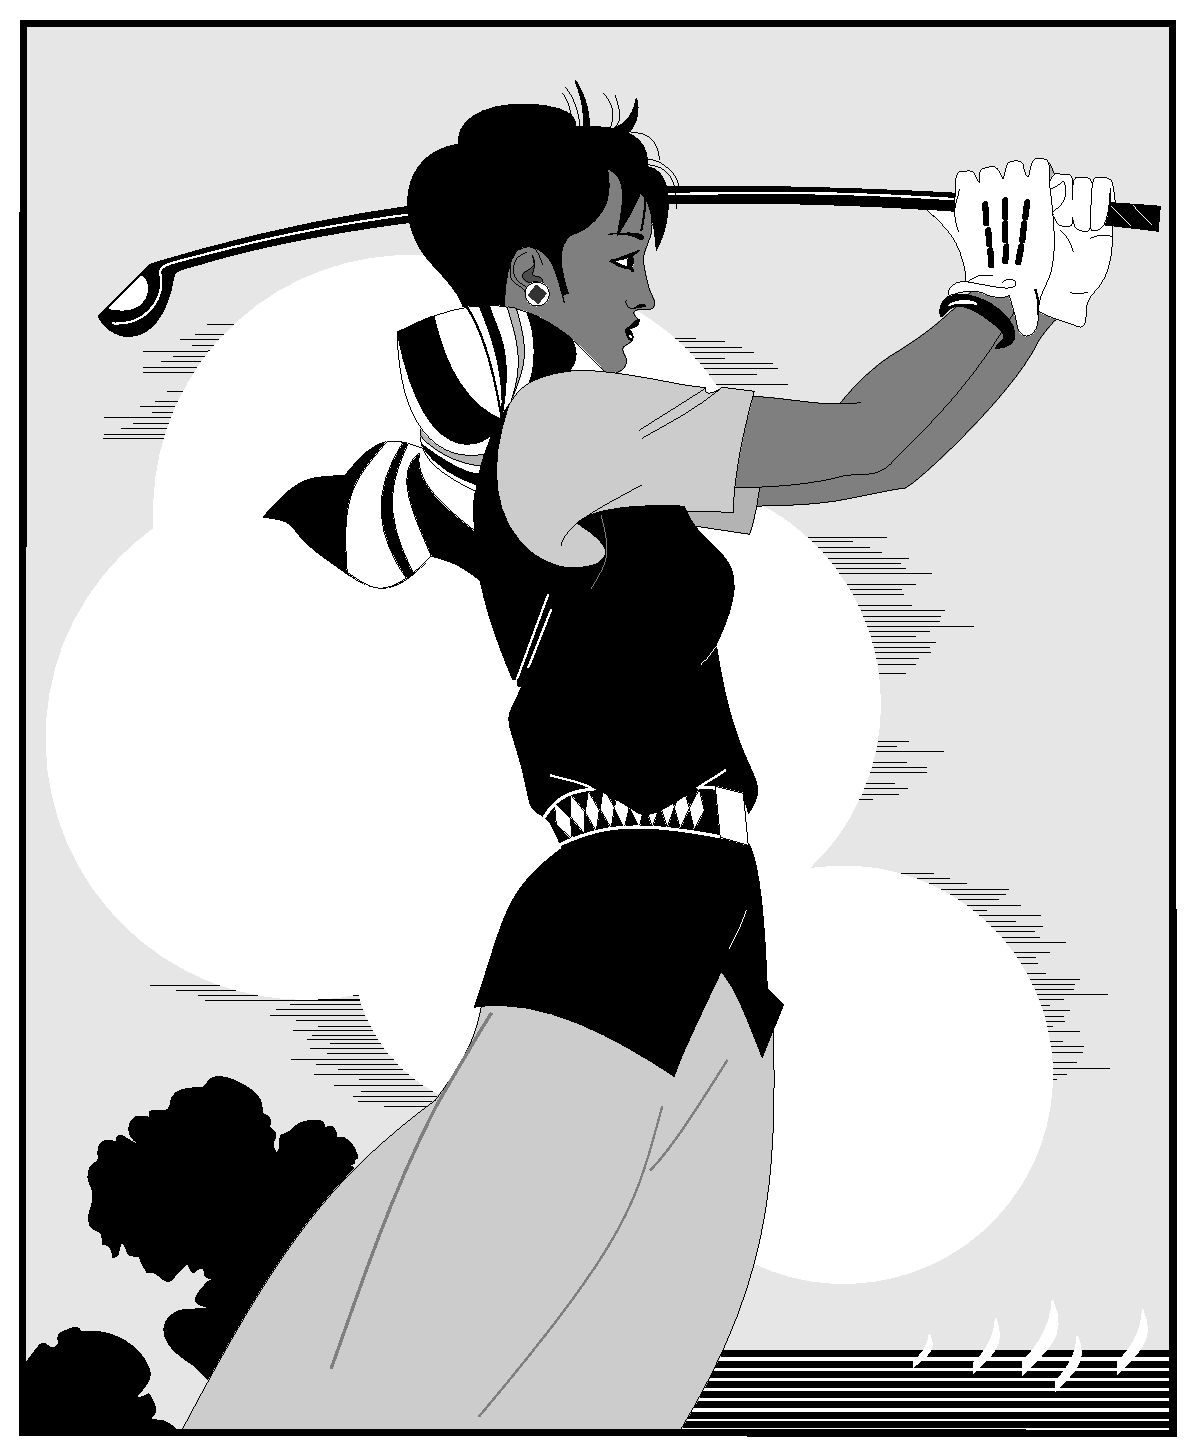
\includegraphics[width = 0.4\textwidth]{golfer}
% \bicaption[golfer1]{}{注意,如果这里字数过长,模板会自动选择最佳字号
% }{Fig.$\!$}{The person playing golf}
% \end{figure}
% \end{latex}
% 单张单图题的格式如下,
% \begin{latex}
% \begin{figure}[h]
% \centering
% 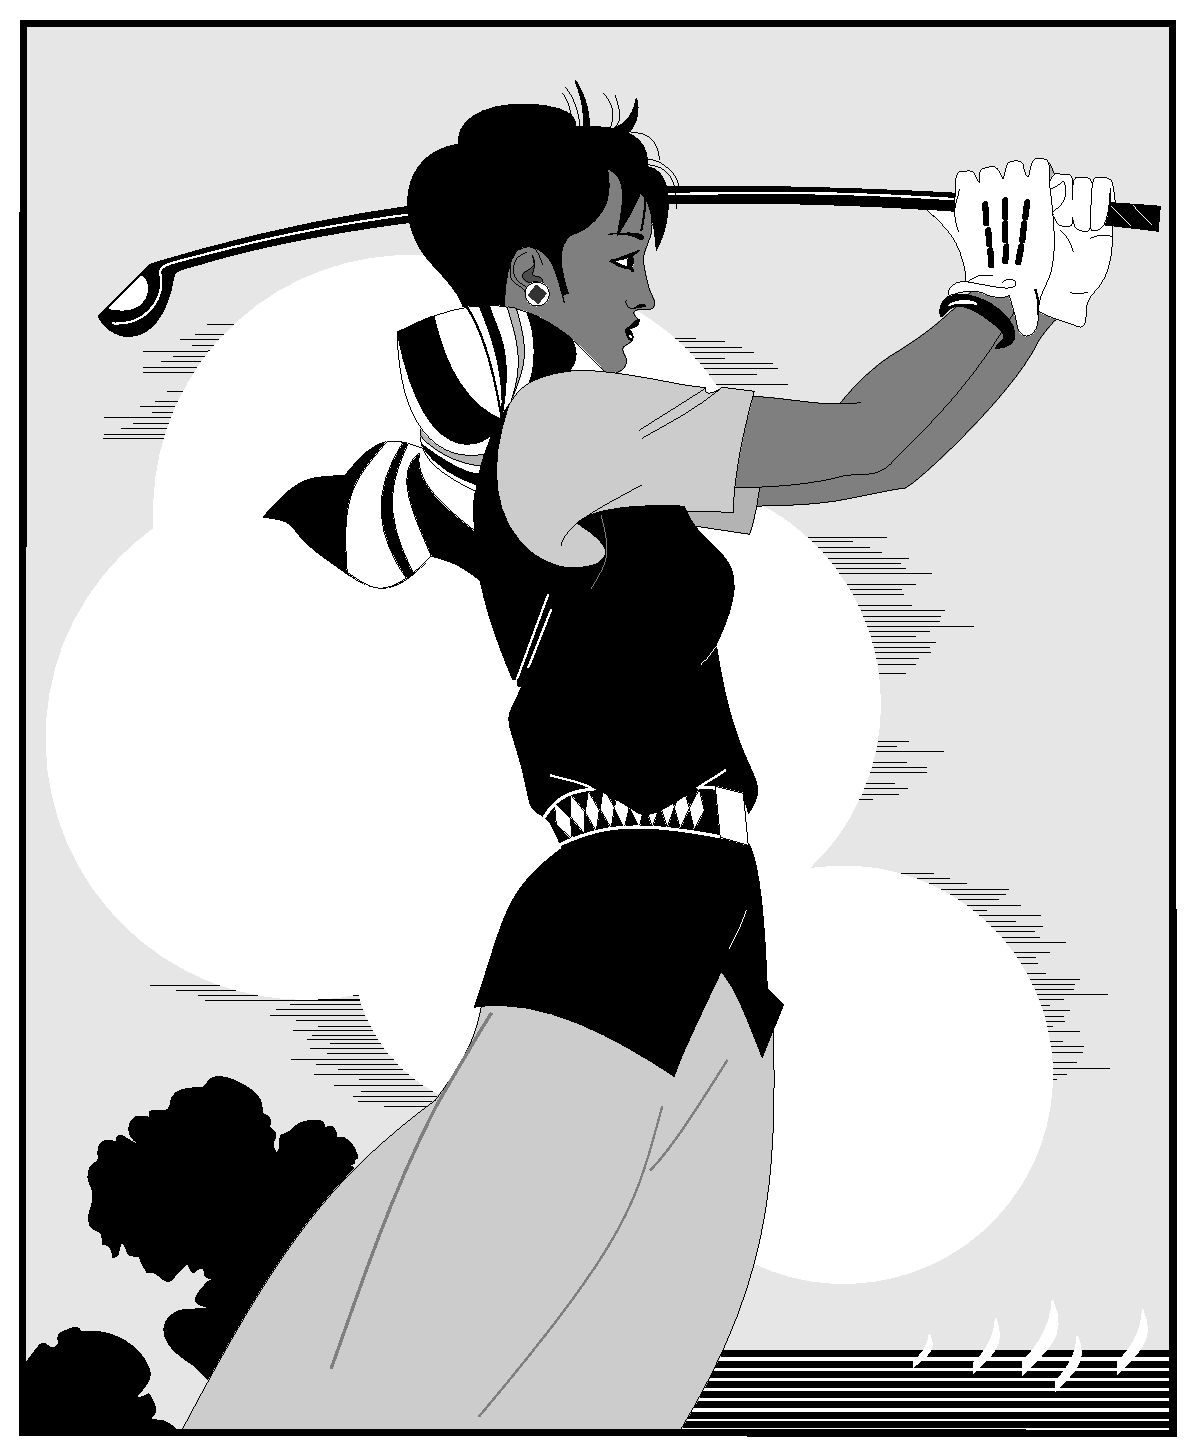
\includegraphics[width = 0.4\textwidth]{golfer}
% \caption{注意,如果这里字数过长,模板会自动选择最佳字号}
% \end{figure}
% \end{latex}
% 带有子图的双语格式,
%
% \subsubsection{公式}
% \subsubsection{数学环境}
% \label{sec:math}
% \hithesis\ 定义了常用的数学环境:
%
% \begin{center}
% \begin{tabular}{*{7}{l}}\toprule
%   axiom & theorem & definition & proposition & lemma & conjecture &\\
%   公理 & 定理 & 定义 & 命题 & 引理 & 猜想 &\\\midrule
%   proof & corollary & example & exercise & assumption & remark & problem \\
%   证明 & 推论 & 例子& 练习 & 假设 & 注释 & 问题\\\bottomrule
% \end{tabular}
% \end{center}
%
% 比如:
% \begin{latex}
% \begin{definition}
%   道千乘之国,敬事而信,节用而爱人,使民以时。
% \end{definition}
% \end{latex}
% 产生(自动编号):
% \medskip
%
% \noindent\framebox[\linewidth][l]{{\heiti 定义~1.1~~~} % {道千乘之国,敬事而信,节用而爱人,使民以时。}}
%
% \smallskip
% 列举出来的数学环境毕竟是有限的,如果想用\emph{胡说}这样的数学环境,那么可以定义:
% \begin{latex}
% \newtheorem{nonsense}{胡说}[chapter]
% \end{latex}
%
% 然后这样使用:
% \begin{latex}
% \begin{nonsense}
%   契丹武士要来中原夺武林秘笈。—— 慕容博
% \end{nonsense}
% \end{latex}
% 产生(自动编号):
%
% \medskip
% \noindent\framebox[\linewidth][l]{{\heiti 胡说~1.1~~~} % {契丹武士要来中原夺武林秘笈。—— 慕容博}}
%
% \subsubsection{算法}
%
% \subsubsection{引用参考文献}
% \DescribeMacro{\inlinecite}
% 学校要求的参考文献引用有两种模式:(1)上标模式。比如``同样的工作有很
% 多$^{[1,2]}$\ldots''。(2)正文模式。比如``文[3] 中详细说明了\ldots''。其中上标
% 模式使用远比正文模式频繁,所以为了符合使用习惯,上标模式仍然用常规
% 的 \cs{cite}\marg{key},而 \cs{inlinecite}\marg{key} 则用来生成正文模式。
%
% 关于参考文献模板推荐使用 \BibTeX,关于中文参考文献需要额外增加一个 Entry:
% \texttt{lang},将其设置为 \texttt{zh} 用来指示此参考文献为中文,以
% 便 \file{hithesis.bst} 处理。如:
% \begin{latex}
% @INPROCEEDINGS{cnproceed,
%   author    = {王重阳 and 黄药师 and 欧阳峰 and 洪七公 and 段皇帝},
%   title     = {武林高手从入门到精通},
%   booktitle = {第~$N$~次华山论剑},
%   year      = 2006,
%   address   = {西安, 中国},
%   month     = sep,
%   lang      = "zh",
% }
%
% @ARTICLE{cnarticle,
%   AUTHOR  = "贾宝玉 and 林黛玉 and 薛宝钗 and 贾探春",
%   TITLE   = "论刘姥姥食量大如牛之现实意义",
%   JOURNAL = "红楼梦杂谈",
%   PAGES   = "260--266",
%   VOLUME  = "224",
%   YEAR    = "1800",
%   LANG    = "zh",
% }
% \end{latex}
%
% 注意如果不需要引用参考文献,请删除 \file{main.tex} 中 \cs{bibliography} 开头的两行,
% 以避免可能的编译错误。
%
% \subsubsection{列表环境}
% \DescribeEnv{itemize}
% \DescribeEnv{enumerate}
% \DescribeEnv{description}
% 为了适合中文习惯,模板将这三个常用的列表环境用 \pkg{enumitem} 进行了纵向间距压
% 缩。一方面清除了多余空间,另一方面用户可以自己指定列表环境的样式(如标签符号,
% 缩进等)。细节请参看 \pkg{enumitem} 文档,此处不再赘述。
% \subsection{后文}
%
% \subsubsection{结论}
% \DescribeEnv{conclusion}
% 结论之后为后文内容。
% \begin{latex}
% \begin{conclusions}
%
% 学位论文的结论作为论文正文的最后一章单独排写,但不加章标题序号。
%
% 结论应是作者在学位论文研究过程中所取得的创新性成果的概要总结,不能与摘要混为一
% 谈。博士学位论文结论应包括论文的主要结果、创新点、展望三部分,在结论中应概括论
% 文的核心观点,明确、客观地指出本研究内容的创新性成果(含新见解、新观点、方法创
% 新、技术创新、理论创新),并指出今后进一步在本研究方向进行研究工作的展望与设想
% 。对所取得的创新性成果应注意从定性和定量两方面给出科学、准确的评价,分(1)、
% (2)、(3)…条列出,宜用“提出了”、“建立了”等词叙述。
%
% \end{conclusions}
% \end{latex}
%
% \subsubsection{参考文献}
% 在后文中的参考文献是自动生成的,不需要用户干预,具体命令在\file{main.tex}中有
% 示例。
%
% \subsubsection{附录}
% \DescribeEnv{appendix}
% 所有的附录都插到这里来。因为附录会更改默认的 chapter 属性,而后面的{\heiti 个人简
%   历}又需要恢复,所以实现为环境可以保证全局的属性不受影响。
% \begin{latex}
% \begin{appendix}
% % -*-coding: utf-8 -*-
%%%%%%%%%%%%%%%%%%%%%%%%%%%%%%%%%%%%%%%%%%%%%%%%%%%%%%%%%
\chapter{带章节的附录}[Full Appendix]%
完整的附录内容,包含章节,公式,图表等

%%%%%%%%%%%%%%%%%%%%%%%%%%%%%%%%%%%%%%%%%%%%%%%%%%%%%%%%%
\section{附录节的内容}[Section in Appendix]
这是附录的节的内容

附录中图的示例:
\begin{figure}[htbp]
\centering
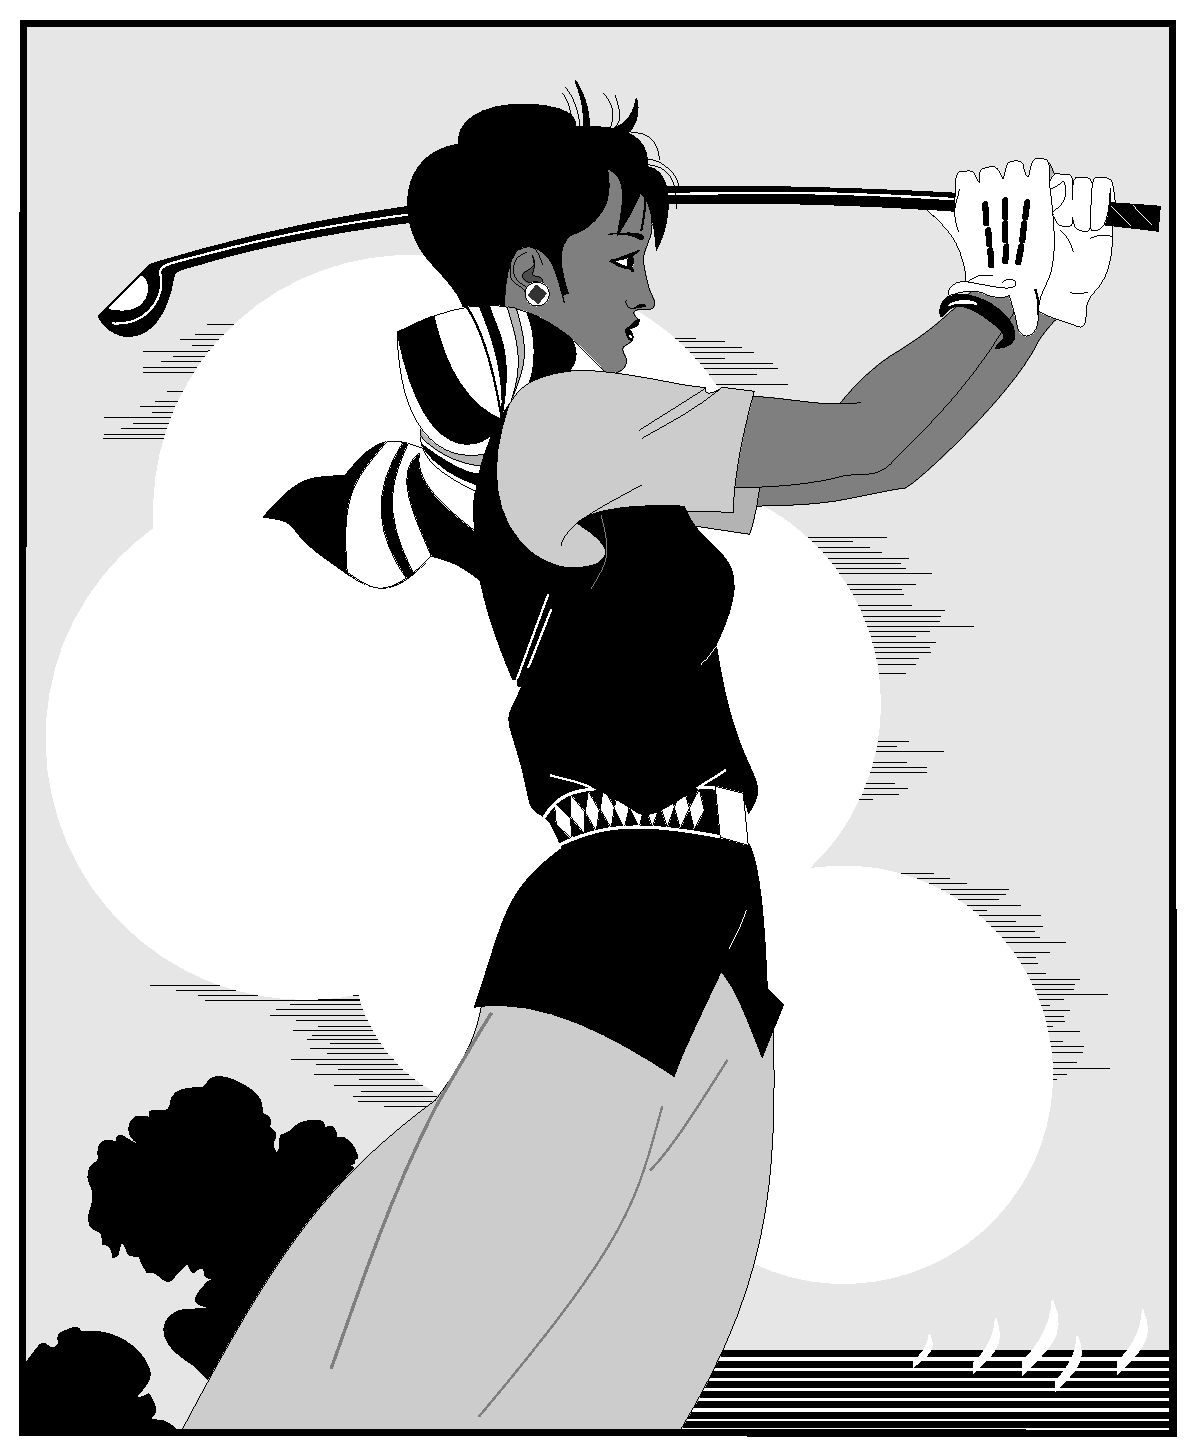
\includegraphics[width = 0.4\textwidth]{golfer}
%\bicaption[golfer5]{}{\xiaosi[0]打高尔夫球的人}{Fig.$\!$}{The person playing golf}\vspace{-1em}
\caption{\xiaosi[0]打高尔夫球的人}
\end{figure}

附录中公式的示例:
\begin{align}
a & = b \times c \\
E & = m c^2
\label{eq}
\end{align}

\chapter{这个星球上最好的免费Linux软件列表}[List of the Best Linux Software in our Planet]
\section*{系统}

\href{http://fvwm.org/}{FVWM 星球最强大的窗口管理器}——推荐

\section*{其他}

\href{https://github.com/goldendict/goldendict}{goldendict 星球最强大的桌面字典}——推荐

\href{http://www.mutt.org/}{mutt 星球最强大的邮件客户端}——推荐

% \end{appendix}
% \end{latex}
%
% \subsubsection{所发表文章}
% \DescribeEnv{publication}
% 虽然在\PGR\UGR\ 中都没有明确规定此处的格式,但按照旧模板PlutoThesis,此处格式
% 非常复杂。此处仍然使用旧模板中的设置方法。
% \begin{latex}
% \begin{publication}
% \noindent\textbf{(一)发表的学术论文}
% \begin{publist}
% \item	XXX,XXX. Static Oxidation Model of Al-Mg/C Dissipation Thermal Protection Materials[J]. Rare Metal Materials and Engineering, 2010, 39(Suppl. 1): 520-524.(SCI~收录,IDS号为~669JS,IF=0.16)
% \item XXX,XXX. 精密超声振动切削单晶铜的计算机仿真研究[J]. 系统仿真学报,2007,19(4):738-741,753.(EI~收录号:20071310514841)
% \item XXX,XXX. 局部多孔质气体静压轴向轴承静态特性的数值求解[J]. 摩擦学学报,2007(1):68-72.(EI~收录号:20071510544816)
% \item XXX,XXX. 硬脆光学晶体材料超精密切削理论研究综述[J]. 机械工程学报,2003,39(8):15-22.(EI~收录号:2004088028875)
% \item XXX,XXX. 基于遗传算法的超精密切削加工表面粗糙度预测模型的参数辨识以及切削参数优化[J]. 机械工程学报,2005,41(11):158-162.(EI~收录号:2006039650087)
% \item XXX,XXX. Discrete Sliding Mode Cintrok with Fuzzy Adaptive Reaching Law on 6-PEES Parallel Robot[C]. Intelligent System Design and Applications, Jinan, 2006: 649-652.(EI~收录号:20073210746529)
% \end{publist}
%
% \noindent\textbf{(二)申请及已获得的专利(无专利时此项不必列出)}
% \begin{publist}
% \item XXX,XXX. 一种温热外敷药制备方案:中国,88105607.3[P]. 1989-07-26.
% \end{publist}
%
% \noindent\textbf{(三)参与的科研项目及获奖情况}
% \begin{publist}
% \item	XXX,XXX. XX~气体静压轴承技术研究, XX~省自然科学基金项目.课题编号:XXXX.
% \item XXX,XXX. XX~静载下预应力混凝土房屋结构设计统一理论. 黑江省科学技术二等奖, 2007.
% \end{publist}
% %\vfill
% %\hangafter=1\hangindent=2em\noindent
% %\setlength{\parindent}{2em}
% \end{publication}
% \end{latex}
%
% \subsubsection{索引}
% \DescribeEnv{ceindex}
% 我工要求中英文双语索引。后文中的自动索引实际上不需要用户干预。
%\begin{latex}
% \begin{ceindex}
%   %如果想要手动加索引,注释掉以下这一样,用wordlist环境
% \printsubindex*
% \end{ceindex}
%\end{latex}
% 手工添加索引的方法不推荐,模板中将去除该功能。
% \subsubsection{授权}
% \DescribeMacro{\authorization}
% 授权页中的签名和日期是需要手写,不需要人工干预。具体示例在\file{main.tex}中。
%\begin{latex}
% \authorization %授权
% %\authorization[saomiao.pdf] %添加扫描页的命令,与上互斥
%\end{latex}
%
% \subsubsection{致谢声明}
% \DescribeEnv{acknowledgement}
% 把致谢做成一个环境更好一些,直接往里面写感谢的话就可以啦!
% \begin{latex}
% \begin{acknowledgement}
%   …
%   感谢\hit\LaTeX\ 论文模板\hithesis\ !
% \end{acknowledgement}
% \end{latex}
%
%
% \subsubsection{简历}
% \DescribeEnv{resume}
% 个人简历。
% 实际上,致谢和个人简历是自由发挥的地区,字体,文体,格式,内容,完全自己决定。
% \begin{latex}
% \begin{resume}
% XXXX~年~XX~月~XX~日出生于~XXXX。
%
% XXXX~年~XX~月考入~XX~大学~XX~院(系)XX~专业,XXXX~年~XX~月本科毕业并获得~XX~学学士学位。
%
% XXXX~年~XX~月------XXXX~年~XX~月在~XX~大学~XX~院(系)XX~学科学习并获得~XX~学硕士学位。
%
% XXXX~年~XX~月------XXXX~年~XX~月在~XX~大学~XX~院(系)XX~学科学习并获得~XX~学博士学位。
%
% 获奖情况:如获三好学生、优秀团干部、X~奖学金等(不含科研学术获奖)。
%
% 工作经历:
% \end{resume}
% \end{latex}
%
% \subsection{其它}
% 模板的配置文件 \file{hithesis.cfg} 中定义了很多固定词汇,一般无须修改。如果有特殊需求,
% 推荐在导言区使用 \cs{renewcommand}。
%
% \StopEventually{\PrintChanges\PrintIndex}
% \clearpage
%
% \section{实现细节}
%
% \subsection{基本信息}
%    \begin{macrocode}
%<cls>\NeedsTeXFormat{LaTeX2e}[1999/12/01]
%<cls>\ProvidesClass{hithesis}
%<cfg>\ProvidesFile{hithesis.cfg}
%<cls|cfg>[2017/08/21 0.0.1 Harbin Institute of Technology]
%    \end{macrocode}
%
% \subsection{定义选项}
% \label{sec:defoption}
%    \begin{macrocode}
%<*cls>
\RequirePackage{ifthen}
\RequirePackage{kvoptions}
\SetupKeyvalOptions{
  family=hit,
  prefix=hit@,
  setkeys=\kvsetkeys}
\newif\ifhit@bachelor
\newif\ifhit@master
\newif\ifhit@doctor
\define@key{hit}{type}{%
  \hit@bachelorfalse
  \hit@masterfalse
  \hit@doctorfalse
  \expandafter\csname hit@#1true\endcsname}
%    \end{macrocode}
% 目录中英文是否用 Arial 字体(默认关闭)。
%    \begin{macrocode}
\DeclareBoolOption[false]{arialtoc}
%    \end{macrocode}
% 章节标题中的英文是否用 Arial 字体(默认打开)。
%    \begin{macrocode}
\DeclareBoolOption[false]{arialtitle}
%    \end{macrocode}
% \option{raggedbottom} 选项(默认关闭)。
%    \begin{macrocode}
\DeclareBoolOption[false]{raggedbottom}
%    \end{macrocode}
% 在脚注标记中使用 \pkg{pifont} 的带圈数字(默认关闭)。
%    \begin{macrocode}
\DeclareBoolOption[false]{pifootnote}
%    \end{macrocode}
% 字体间距设置(默认关闭)。
%    \begin{macrocode}
\DeclareBoolOption[false]{glue}
%    \end{macrocode}
% 文科生四级目录设置(默认关闭)。
%    \begin{macrocode}
\DeclareBoolOption[false]{tocfour}
%    \end{macrocode}
% 目录中“目录”位置是否空行(默认开启)。
%    \begin{macrocode}
\DeclareBoolOption[true]{tocblank}
%    \end{macrocode}
% 章标题是否悬挂居中(默认开启)
%    \begin{macrocode}
\DeclareBoolOption[true]{chapterhang}
%    \end{macrocode}
% 是否是全日制学生(默认是)。
%    \begin{macrocode}
\DeclareBoolOption[true]{fulltime}
%    \end{macrocode}
% 是否有子标题(默认是)。
%    \begin{macrocode}
\DeclareBoolOption[false]{subtitle}
%    \end{macrocode}
% 是否开启debug模式(默认否)。如果开启,载入显示行号等的包,只为开发调试用。
%    \begin{macrocode}
\DeclareBoolOption[false]{debug}
%    \end{macrocode}
% 是否使用新的版心设置(默认否)。
%    \begin{macrocode}
\DeclareBoolOption[false]{newgeometry}
%    \end{macrocode}
% 是否使用右开页(默认否)。
%    \begin{macrocode}
\DeclareBoolOption[false]{openright}
%    \end{macrocode}
% 声明字体选项。
%    \begin{macrocode}
\DeclareStringOption{fontset}
%    \end{macrocode}
% 将其余选项默认传递给 \pkg{ctexbook}。
%    \begin{macrocode}
\DeclareDefaultOption{\PassOptionsToClass{\CurrentOption}{ctexbook}}
%    \end{macrocode}
% 解析用户传递过来的选项,并加载 \pkg{ctexbook}。
%    \begin{macrocode}
\ProcessKeyvalOptions*
%    \end{macrocode}
% 使用 \XeTeX\ 引擎时,\pkg{fontspec} 宏包会被 \pkg{xeCJK} 自动调用。传递
% 给 \pkg{fontspec} 宏包 \option{no-math} 选项,避免部分数学符号字体自动调整
% 为 CMR。其他引擎下没有这个问题,这一行会被无视。
%    \begin{macrocode}
\PassOptionsToPackage{no-math}{fontspec}
%    \end{macrocode}
% 载入单双面打印设置,本、硕单面,博士双面。
%    \begin{macrocode}
\ifhit@bachelor
\PassOptionsToClass{oneside}{book}
\fi
\ifhit@master
\PassOptionsToClass{oneside}{book}
\fi
\ifhit@doctor
\PassOptionsToClass{twoside}{book}
\fi
%    \end{macrocode}
% 设置字体。由于宋体没有粗体,且我工模板的标题要求使用粗宋体,于是面临CTeX的经典
% 的伪粗体bug:“首次出现伪粗体字体之后的正常字体无法复制”。但如果使用自带宋体的
% 思源字体,那么不必使用伪粗体。
%    \begin{macrocode}
\ifthenelse%
{\equal{\hit@fontset}{}}%
{%
  \PassOptionsToPackage{AutoFakeBold=2}{xeCJK}
}%
{%
  \ifthenelse%
  {\equal{\hit@fontset}{siyuan}}%
  {\relax}%
  {%
    \PassOptionsToPackage{AutoFakeBold=2}{xeCJK}
  }%
  \PassOptionsToClass{fontset=\hit@fontset}{ctexbook}
}%
%    \end{macrocode}
% 使用 \pkg{ctexbook} 类,优于调用 \pkg{ctex} 宏包。
%    \begin{macrocode}
\LoadClass[a4paper,openany,UTF8,zihao=-4,scheme=plain]{ctexbook}
%    \end{macrocode}
% 用户至少要提供一个选项,指定论文类型。
%    \begin{macrocode}
\ifhit@bachelor\relax\else
  \ifhit@master\relax\else
    \ifhit@doctor\relax\else
        \ClassError{hithesis}%
                   {Please specify thesis type in option: \MessageBreak
                    type=[bachelor | master | doctor]}{}
      \fi
  \fi
\fi
%    \end{macrocode}
%
% \subsection{装载宏包}
% \label{sec:loadpackage}
%
% 引用的宏包和相应的定义。
%    \begin{macrocode}
\RequirePackage{etoolbox}
\RequirePackage{ifxetex}
\ifxetex
\else
        \ClassError{hithesis}%
                   {Please use: \MessageBreak
                    xelatex}{}
\fi
\RequirePackage{xparse}
%    \end{macrocode}
%
% \AmSTeX\ 宏包,用来排出更加漂亮的公式。
%    \begin{macrocode}
\RequirePackage{amsmath}
%    \end{macrocode}
%
% \pkg{newtx} 设置 Times New Roman,Helvetica。
%    \begin{macrocode}
\RequirePackage[defaultsups]{newtxtext}
\RequirePackage{newtxmath}
%    \end{macrocode}
% \pkg{newtx} 的 Mono 字体虽然很好看,但在论文中不常见。学校虽未要求 Mono 字体,
% 还是选择常见的 Courier 字体。由于比较新的实现 \TeX\ Gyre Cursor 会修
% 改\cs{bfdefault},导致中文加粗出问题,所以选用标准 \pkg{courier}。
%    \begin{macrocode}
\RequirePackage{courier}
%    \end{macrocode}
% 图形支持宏包。
%    \begin{macrocode}
\RequirePackage{graphicx}
%    \end{macrocode}
% \pkg{pdfpages} 宏包便于我们插入扫描后的授权页和声明页 PDF 文档。
%    \begin{macrocode}
\RequirePackage{pdfpages}
\includepdfset{fitpaper=true}
%    \end{macrocode}
% 更好的列表环境。
%    \begin{macrocode}
\RequirePackage{enumitem}       %使用enumitem宏包,改变列表项的格式
\RequirePackage{environ}
%    \end{macrocode}
% 禁止 \LaTeX 自动调整多余的页面底部空白,并保持脚注仍然在底部。
% 脚注按页编号。
%    \begin{macrocode}
\ifhit@raggedbottom
  \RequirePackage[bottom,perpage,hang]{footmisc}
  \raggedbottom
\else
  \RequirePackage[perpage,hang]{footmisc}
\fi
%    \end{macrocode}
% 脚注格式。
%    \begin{macrocode}
\ifhit@pifootnote
  \RequirePackage{pifont}
\fi
%    \end{macrocode}
% 利用 \pkg{CJKfntef} 实现汉字的下划线和盒子内两段对齐,并可以避免
% \cs{makebox}\oarg{width}\oarg{s} 可能产生的 underful boxes。
%    \begin{macrocode}
\RequirePackage{CJKfntef}
%    \end{macrocode}
% 定理类环境宏包,其中 \pkg{amsmath} 选项用来兼容 \AmSTeX\ 的宏包
%    \begin{macrocode}
\RequirePackage[amsmath,thmmarks,hyperref]{ntheorem}
%    \end{macrocode}
% 表格控制
%    \begin{macrocode}
\RequirePackage{longtable}
%    \end{macrocode}
% 使用三线表:\cs{toprule},\cs{midrule},\cs{bottomrule}。
%    \begin{macrocode}
\RequirePackage{booktabs}
%    \end{macrocode}
% 参考文献引用宏包。
%    \begin{macrocode}
\RequirePackage[sort&compress]{natbib}
%    \end{macrocode}
% 生成有书签的 pdf 及其开关,请结合 gbk2uni 避免书签乱码。
%    \begin{macrocode}
\RequirePackage{hyperref}
\hypersetup{%
  CJKbookmarks=true,
  linktoc=all,
  bookmarksnumbered=true,
  bookmarksopen=true,
  bookmarksopenlevel=1,
  breaklinks=true,
  colorlinks=false,
  plainpages=false,
  pdfborder=0 0 0}
%    \end{macrocode}
% 设置 url 样式,与上下文一致
%    \begin{macrocode}
\urlstyle{same}
%    \end{macrocode}
%
% \subsection{页面设置}
% \label{sec:layout}
% 本来这部分应该是最容易设置的,但根据我工\PGR\ 的3.8,3.4,3.2节的版芯矛盾,此处
% 设置两种版芯。
%    \begin{macrocode}
\ifhit@debug\RequirePackage[showframe]{geometry}\else\RequirePackage{geometry}\fi
\geometry{%根据PlutoThesis 原版定义而来
  a4paper, % 210 * 297mm
  hcentering,
  ignoreall,
  nomarginpar,
}
\ifhit@newgeometry%
\geometry{
  centering,
  text={150true mm,240true mm},
  left=30true mm,
  head=5true mm,
  headsep=0true mm,
  footskip=0true mm,
  foot=0true mm
}
\else%
\geometry{%根据PlutoThesis 原版定义而来
  text={150true mm,224true mm},
  top=35.5true mm,
  left=30true mm,
  head=5true mm,
  headsep=2.5true mm,
  foot=8.5true mm
}
\fi
%    \end{macrocode}
%    载入显示行号的包。
%    \begin{macrocode}
\ifhit@debug%
\RequirePackage{layout}
\RequirePackage{lineno}
\fi
%    \end{macrocode}
% 利用 \pkg{fancyhdr} 设置页眉页脚。
%    \begin{macrocode}
\RequirePackage{fancyhdr}
%</cls>
%    \end{macrocode}
%
% \subsection{主文档格式}
% \label{sec:mainbody}
%
% \subsubsection{Three matters}
% \begin{macro}{\cleardoublepage}
% 对于 \textsl{openright} 选项,必须保证章首页右开,且如果前章末页无内容须
% 清空其页眉页脚。
%    \begin{macrocode}
%<*cls>
\let\hit@cleardoublepage\cleardoublepage
\newcommand{\hit@clearemptydoublepage}{%
  \clearpage{\pagestyle{hit@empty}\hit@cleardoublepage}}
\let\cleardoublepage\hit@clearemptydoublepage
%    \end{macrocode}
% \end{macro}
%
% \begin{macro}{\frontmatter}
% \begin{macro}{\mainmatter}
% \begin{macro}{\backmatter}
% 我们的单面和双面模式与常规的不太一样。
% \changes{v2.5.1}{2006/05/23}{本科正文之后页码即用罗马数字,研究生不变。}
% \changes{v2.5.3}{2006/06/03}{第一章永远右开。}
% \changes{v4.4}{2008/05/30}{本科正文后的页码延续前面的阿拉伯数字,不再用罗马数
% 字。}
% \changes{v4.4}{2008/05/30}{本科取消了所有页眉。}
%    \begin{macrocode}
\renewcommand\frontmatter{%
  \if@openright\cleardoublepage\else\clearpage\fi
  \@mainmatterfalse
  \pagenumbering{Roman}
  \pagestyle{hit@empty}}
\renewcommand\mainmatter{%
  \if@openright\cleardoublepage\else\clearpage\fi
  \@mainmattertrue
  \pagenumbering{arabic}
  \ifhit@bachelor\pagestyle{hit@plain}\else\pagestyle{hit@headings}\fi}
\renewcommand\backmatter{%
  \if@openright\cleardoublepage\else\clearpage\fi
  \@mainmattertrue}
%</cls>
%    \end{macrocode}
% \end{macro}
% \end{macro}
% \end{macro}
%
% \subsubsection{字体}
% \label{sec:font}
% \begin{macro}{\normalsize}
% 正文小四号 (12bp) 字,行距为固定值 20 bp。
%    \begin{macrocode}
%<*cls>
\renewcommand\normalsize{%
  \@setfontsize\normalsize{12bp}{20bp}%
  \abovedisplayskip=20bp \@plus 2bp \@minus 2bp
  \abovedisplayshortskip=20bp \@plus 2bp \@minus 2bp
  \belowdisplayskip=\abovedisplayskip
  \belowdisplayshortskip=\abovedisplayshortskip}
%    \end{macrocode}
% \end{macro}
%
% WORD 中的字号对应该关系如下(1bp = 72.27/72 pt):
% \begin{center}
% \begin{tabular}{llll}
% \toprule
% 初号 & 42bp & 14.82mm & 42.1575pt \\
% 小初 & 36bp & 12.70mm & 36.135 pt \\
% 一号 & 26bp & 9.17mm & 26.0975pt \\
% 小一 & 24bp & 8.47mm & 24.09pt \\
% 二号 & 22bp & 7.76mm & 22.0825pt \\
% 小二 & 18bp & 6.35mm & 18.0675pt \\
% 三号 & 16bp & 5.64mm & 16.06pt \\
% 小三 & 15bp & 5.29mm & 15.05625pt \\
% 四号 & 14bp & 4.94mm & 14.0525pt \\
% 小四 & 12bp & 4.23mm & 12.045pt \\
% 五号 & 10.5bp & 3.70mm & 10.59375pt \\
% 小五 & 9bp & 3.18mm & 9.03375pt \\
% 六号 & 7.5bp & 2.56mm & \\
% 小六 & 6.5bp & 2.29mm & \\
% 七号 & 5.5bp & 1.94mm & \\
% 八号 & 5bp & 1.76mm & \\\bottomrule
% \end{tabular}
% \end{center}
%
% \begin{macro}{\hit@def@fontsize}
% \changes{v2.6.2}{2006/06/18}{引入此命令重新定义字号。}
% 根据习惯定义字号。用法:
%
% \cs{hit@def@fontsize}\marg{字号名称}\marg{磅数}
%
% 避免了字号选择和行距的紧耦合。所有字号定义时为单倍行距,并提供选项指定行距倍数。
% \changes{v5.2.3}{2016/02/13}{改写字体定义命令。}
%    \begin{macrocode}
\def\hit@def@fontsize#1#2{%
  \expandafter\newcommand\csname #1\endcsname[1][1.3]{%
    \fontsize{#2}{##1\dimexpr #2}\selectfont}}
%    \end{macrocode}
% \end{macro}
%
% \begin{macro}{\chuhao}
% \begin{macro}{\xiaochu}
% \begin{macro}{\yihao}
% \begin{macro}{\xiaoyi}
% \begin{macro}{\erhao}
% \begin{macro}{\xiaoer}
% \begin{macro}{\sanhao}
% \begin{macro}{\xiaosan}
% \begin{macro}{\sihao}
% \begin{macro}{\banxiaosi}
% \begin{macro}{\xiaosi}
% \begin{macro}{\dawu}
% \begin{macro}{\wuhao}
% \begin{macro}{\xiaowu}
% \begin{macro}{\liuhao}
% \begin{macro}{\xiaoliu}
% \begin{macro}{\qihao}
% \begin{macro}{\bahao}
% 一组字号定义。TODO:用 \cs{zihao} 替代。
%    \begin{macrocode}
\hit@def@fontsize{chuhao}{42bp}
\hit@def@fontsize{xiaochu}{36bp}
\hit@def@fontsize{yihao}{26bp}
\hit@def@fontsize{xiaoyi}{24bp}
\hit@def@fontsize{erhao}{22bp}
\hit@def@fontsize{xiaoer}{18bp}
\hit@def@fontsize{sanhao}{16bp}
\hit@def@fontsize{xiaosan}{15bp}
\hit@def@fontsize{sihao}{14bp}
\hit@def@fontsize{banxiaosi}{13bp}
\hit@def@fontsize{xiaosi}{12bp}
\hit@def@fontsize{dawu}{11bp}
\hit@def@fontsize{wuhao}{10.5bp}
\hit@def@fontsize{xiaowu}{9bp}
\hit@def@fontsize{liuhao}{7.5bp}
\hit@def@fontsize{xiaoliu}{6.5bp}
\hit@def@fontsize{qihao}{5.5bp}
\hit@def@fontsize{bahao}{5bp}
%</cls>
%    \end{macrocode}
% \end{macro}
% \end{macro}
% \end{macro}
% \end{macro}
% \end{macro}
% \end{macro}
% \end{macro}
% \end{macro}
% \end{macro}
% \end{macro}
% \end{macro}
% \end{macro}
% \end{macro}
% \end{macro}
% \end{macro}
% \end{macro}
% \end{macro}
% \end{macro}
%
%
% \subsubsection{页眉页脚}
% \label{sec:headerfooter}
%
% 定义页眉和页脚。
% \begin{macro}{\ps@hit@empty}
% \begin{macro}{\ps@hit@plain}
% \begin{macro}{\ps@hit@headings}
% \changes{v2.0}{2005/12/18}{以前的太乱了,重新整理过清晰多了。}
% \changes{v2.1}{2006/03/01}{彻底放弃 fancyhdr,定义自己的样式。}
% \changes{v2.5}{2006/05/13}{本科的奇偶页眉不同。}
% \changes{v2.5}{2006/05/20}{增加 empty 页面样式。}
% \changes{v4.7}{2012/05/29}{本科页码用小五号字。}
% \changes{v5.0.0}{2015/12/20}{利用 \pkg{fancyhdr} 设置页眉页脚。}
% 定义三种页眉页脚格式:
% \begin{itemize}
% \item \texttt{hit@empty}:页眉页脚都没有
% \item \texttt{hit@plain}:只显示页脚的页码。\cs{chapter} 自动调用
% \cs{thispagestyle\{hit@plain\}}。
% \item \texttt{hit@headings}:页眉页脚同时显示
% \end{itemize}
%    \begin{macrocode}
%<*cls>
\fancypagestyle{hit@empty}{%
  \fancyhf{}
  \renewcommand{\headrulewidth}{0pt}
  \renewcommand{\footrulewidth}{0pt}}
\fancypagestyle{hit@plain}{%
  \fancyhead{}
  \fancyfoot[C]{\xiaowu\thepage}
  \renewcommand{\headrulewidth}{0pt}
  \renewcommand{\footrulewidth}{0pt}}
\fancypagestyle{hit@headings}{%
  \fancyhead{}
  \fancyhead[C]{\wuhao\normalfont\leftmark}
  \fancyfoot{}
  \fancyfoot[C]{\wuhao\thepage}
  \renewcommand{\headrulewidth}{0.4pt}
  \renewcommand{\footrulewidth}{0pt}}
%</cls>
%    \end{macrocode}
% \end{macro}
% \end{macro}
% \end{macro}
%
%
% \subsubsection{段落}
% \label{sec:paragraph}
%
% 全文首行缩进 2 字符,标点符号用全角
%    \begin{macrocode}
%<*cls>
\ctexset{%
  punct=quanjiao,
  space=auto,
  autoindent=true}
%    \end{macrocode}
%
% 利用 \pkg{enumitem} 命令调整默认列表环境间的距离,以符合中文习惯。
% \changes{v2.5.2}{2006/06/01}{更改默认列表距离。}
%    \begin{macrocode}
\setlist{nosep}
%</cls>
%    \end{macrocode}
%
%
% \subsubsection{脚注}
% \label{sec:footnote}
% 脚注符合中文习惯,数字带圈。
% \changes{v2.1}{2006/03/01}{让脚注它悬挂起来,而且中文中用上标,脚注中用正体。}
% \changes{v2.5}{2006/05/13}{修正 minipage 中的脚注。}
% \begin{macro}{\hit@textcircled}
% \changes{v2.5.1}{2006/05/21}{脚注编号使用 \cs{textcircled} 命令,每页允许至多 99 个。}
% \changes{v5.2.2}{2016/02/01}{脚注编号每页允许至多 9 个。}
% 生成带圈的脚注数字,最多处理到 10。
%    \begin{macrocode}
%<*cls>
\def\hit@textcircled#1{%
  \ifnum\value{#1} >9
    \ClassError{hithesis}%
      {Too many footnotes in this page.}{Keep footnote less than 10.}
  \fi
  \ifhit@pifootnote%
    \ding{\the\numexpr\value{#1}+171\relax}%
  \else%
    \textcircled{\xiaoliu\arabic{#1}}%
  \fi}
\renewcommand{\thefootnote}{\hit@textcircled{footnote}}
\renewcommand{\thempfootnote}{\hit@textcircled{mpfootnote}}
%    \end{macrocode}
% \end{macro}
%
% 定义脚注分割线,字号(宋体小五),以及悬挂缩进(1.5字符)。
%    \begin{macrocode}
\def\footnoterule{\vskip-3\p@\hrule\@width0.3\textwidth\@height0.4\p@\vskip2.6\p@}
\let\hit@footnotesize\footnotesize
\renewcommand\footnotesize{\hit@footnotesize\xiaowu[1.5]}
\footnotemargin1.5em\relax
%    \end{macrocode}
%
% \cs{@makefnmark} 默认是上标样式,而在脚注部分要求为正文大小。利用\cs{patchcmd}
% 动态调整 \cs{@makefnmark} 的定义。
% \changes{v2.6}{2006/06/09}{脚注改成 1.5 倍行距,漂亮。}
% \changes{v5.2.2}{2016/02/01}{基于 \pkg{footmisc} 来设置不同位置 footnote
% marker 样式。}
%    \begin{macrocode}
\let\hit@makefnmark\@makefnmark
\def\hit@@makefnmark{\hbox{{\normalfont\@thefnmark}}}
\pretocmd{\@makefntext}{\let\@makefnmark\hit@@makefnmark}{}{}
\apptocmd{\@makefntext}{\let\@makefnmark\hit@makefnmark}{}{}
%</cls>
%    \end{macrocode}
%
%
% \subsubsection{数学相关}
% \label{sec:equation}
% 允许太长的公式断行、分页等。
%    \begin{macrocode}
%<*cls>
\allowdisplaybreaks[4]
\renewcommand\theequation{\ifnum \c@chapter>\z@ \thechapter-\fi\@arabic\c@equation}
%    \end{macrocode}
%
% 公式距前后文的距离由 4 个参数控制,参见 \cs{normalsize} 的定义。
%
% \changes{v2.5.1}{2006/05/24}{本科公式编号前添加\textbf{公式}二字。需要修 \pkg{amsmath} 极其深的一个命令。}
% \changes{v2.5.1}{2006/05/24}{教务处居然要本科论文公式全文编号!}
% \changes{v2.5.2}{2006/05/29}{上一个版本忘了把研究生的公式编号排除。}
% \changes{v3.0}{2007/05/12}{本科公式又要取消全文统一编号了。}
% 本科的公式编号要求很诡异,不得不修改 \pkg{amsmath} 中很深的一个命令 \cs{tagform@}。
% \changes{v2.6.2}{2006/06/19}{根据不同论文格式显示不同公式编号,并自动加入索引。}
% \changes{v4.2}{2008/01/23}{\cs{eqref} 加括号。}
% 同时为了让 \pkg{amsmath} 的 \cs{tag*} 命令得到正确的格式,我们必须修改这些代
% 码。\cs{make@df@tag} 是定义 \cs{tag*} 和 \cs{tag} 内部命令的。
% \cs{make@df@tag@@} 处理 \cs{tag*},我们就改它!
% \begin{latex}
% \def\make@df@tag{\@ifstar\make@df@tag@@\make@df@tag@@@}
% \def\make@df@tag@@#1{%
%   \gdef\df@tag{\maketag@@@{#1}\def\@currentlabel{#1}}}
% \end{latex}
% \changes{v4.4}{2008/05/30}{本科论文终于去掉了\textbf{公式}二字。}
% \changes{v4.4.4}{2008/06/12}{修复了一个从 v4.3 升级到 v4.4 过程中的丢失公式索引的 bug,原修改代码保留备忘。}
% \changes{v5.2.3}{2016/02/13}{安全注释本科公式部分。}
%    \begin{macrocode}
\def\make@df@tag{\@ifstar\hit@make@df@tag@@\make@df@tag@@@}
\def\hit@make@df@tag@@#1{\gdef\df@tag{\hit@maketag{#1}\def\@currentlabel{#1}}}
\iffalse
\ifhit@bachelor
  \def\hit@maketag#1{\maketag@@@{%
    (\ignorespaces\text{\equationname\hskip0.5em}#1\unskip\@@italiccorr)}}
  \def\tagform@#1{\maketag@@@{%
    (\ignorespaces\text{\equationname\hskip0.5em}#1\unskip\@@italiccorr)\equcaption{#1}}}
\fi
\fi
\def\hit@maketag#1{\maketag@@@{(\ignorespaces #1\unskip\@@italiccorr)}}
\def\tagform@#1{\maketag@@@{(\ignorespaces #1\unskip\@@italiccorr)\equcaption{#1}}}
%    \end{macrocode}
% 修改 \cs{tagform} 会影响 \cs{eqref}。
%    \begin{macrocode}
\renewcommand{\eqref}[1]{\textup{(\ref{#1})}}
%</cls>
%    \end{macrocode}
%
% 定理标题使用黑体,正文使用宋体,冒号隔开。
% \changes{v2.6.2}{2006/06/17}{增加问题和猜想两个数学环境。}
% \changes{v4.2}{2008/03/07}{调整证明环境的编号和结尾的方块。}
% \changes{v5.0.0}{2015/04/18}{修正定理字样为黑体 (\#104)。}
% \changes{v5.3.2}{2017/05/01}{定理环境格式设置(环境标题和环境正文字体设置)统一放置到 .cfg 文件中。}
%    \begin{macrocode}
%<*cfg>
\theorembodyfont{\normalfont}
\theoremheaderfont{\normalfont\heiti}
\theoremsymbol{\ensuremath{\square}}
\newtheorem*{proof}{证明}
\theoremstyle{plain}
\theoremsymbol{}
\theoremseparator{:}
\newtheorem{assumption}{假设}[chapter]
\newtheorem{definition}{定义}[chapter]
\newtheorem{proposition}{命题}[chapter]
\newtheorem{lemma}{引理}[chapter]
\newtheorem{theorem}{定理}[chapter]
\newtheorem{axiom}{公理}[chapter]
\newtheorem{corollary}{推论}[chapter]
\newtheorem{exercise}{练习}[chapter]
\newtheorem{example}{例}[chapter]
\newtheorem{remark}{注释}[chapter]
\newtheorem{problem}{问题}[chapter]
\newtheorem{conjecture}{猜想}[chapter]
%</cfg>
%    \end{macrocode}
%
% \subsubsection{浮动对象以及表格}
% \label{sec:float}
% 设置浮动对象和文字之间的距离
% \changes{v2.6}{2006/06/09}{增加 \cs{floatsep},\cs{@fptop},\cs{@fpsep} 和 \cs{@fpbot}。}
%    \begin{macrocode}
%<*cls>
\setlength{\floatsep}{20bp \@plus4pt \@minus1pt}
\setlength{\intextsep}{20bp \@plus4pt \@minus2pt}
\setlength{\textfloatsep}{20bp \@plus4pt \@minus2pt}
\setlength{\@fptop}{0bp \@plus1.0fil}
\setlength{\@fpsep}{12bp \@plus2.0fil}
\setlength{\@fpbot}{0bp \@plus1.0fil}
%    \end{macrocode}
%
% 下面这组命令使浮动对象的缺省值稍微宽松一点,从而防止幅度对象占据过多的文本页面,
% 也可以防止在很大空白的浮动页上放置很小的图形。
%    \begin{macrocode}
\renewcommand{\textfraction}{0.15}
\renewcommand{\topfraction}{0.85}
\renewcommand{\bottomfraction}{0.65}
\renewcommand{\floatpagefraction}{0.60}
%    \end{macrocode}
%
% 定制浮动图形和表格标题样式
% \begin{itemize}
%   \item 图表标题字体为 11pt, 这里写作大五号
%   \item 去掉图表号后面的冒号。图序与图名文字之间空一个汉字符宽度。
%   \item 图:caption 在下,段前空 6 磅,段后空 12 磅
%   \item 表:caption 在上,段前空 12 磅,段后空 6 磅
% \end{itemize}
% \changes{v2.4}{2006/04/14}{表格内容为 11 磅。}
% \changes{v2.4}{2006/04/14}{图表标题左对齐,取消原先漂亮的 hang 模式。}
% \changes{v2.5}{2006/05/13}{标题上下间距重调,以前没有考虑 \cs{intextsep} 的影响。}
% \changes{v2.5.1}{2006/05/23}{增加 \pkg{subfigure} 和 \pkg{subtable} 的 caption 配置。}
% \changes{v2.5.1}{2006/05/24}{重新定义表格默认字体。}
% \changes{v2.5.3}{2006/06/07}{不管 caption 出现在什么位置,\cs{aboveskip} 总是出现在标题和浮动体之间的距离。}
% \changes{v4.3}{2008/03/11}{子图引用时加括号。}
% \changes{v5.0.0}{2015/06/27}{本科附录图表编号用-不用.(如图A-1,表A-2)。}
%    \begin{macrocode}
\ifhit@bachelor
  \g@addto@macro\appendix{\renewcommand*{\thefigure}{\thechapter-\arabic{figure}}}
  \g@addto@macro\appendix{\renewcommand*{\thetable}{\thechapter-\arabic{table}}}
\fi
\let\old@tabular\@tabular
\def\hit@tabular{\dawu[1.5]\old@tabular}
\DeclareCaptionLabelFormat{hit}{{\dawu[1.5]\normalfont #1~#2}}
\DeclareCaptionLabelSeparator{hit}{\hspace{1em}}
\DeclareCaptionFont{hit}{\dawu[1.5]}
\captionsetup{labelformat=hit,labelsep=hit,font=hit}
\captionsetup[table]{position=top,belowskip={12bp-\intextsep},aboveskip=6bp}
\captionsetup[figure]{position=bottom,belowskip={12bp-\intextsep},aboveskip=6bp}
\captionsetup[sub]{font=hit,skip=6bp}
\renewcommand{\thesubfigure}{(\alph{subfigure})}
\renewcommand{\thesubtable}{(\alph{subtable})}
% \renewcommand{\p@subfigure}{:}
%    \end{macrocode}
% 我们采用 \pkg{longtable} 来处理跨页的表格。同样我们需要设置其默认字体为五号。
% \changes{v2.5.3}{2006/06/08}{增加对 \pkg{longtable} 的处理。}
% \changes{v4.5.1}{2009/01/06}{太好了,不用处理 \pkg{longtable} 的 \cs{caption}
% 了。}
%    \begin{macrocode}
\let\hit@LT@array\LT@array
\def\LT@array{\dawu[1.5]\hit@LT@array} % set default font size
%    \end{macrocode}
%
% \begin{macro}{\hlinewd}
% 简单的表格使用三线表推荐用 \cs{hlinewd}。如果表格比较复杂还是用 \pkg{booktabs} 的命
% 令好一些。
%    \begin{macrocode}
\def\hlinewd#1{%
  \noalign{\ifnum0=`}\fi\hrule \@height #1 \futurelet
    \reserved@a\@xhline}
%</cls>
%    \end{macrocode}
% \end{macro}
%
%
% \subsubsection{章节标题}
% \label{sec:theor}
% \changes{v2.5}{2006/05/19}{增加索引名称定义。}
%    \begin{macrocode}
%<*cfg>
\ctexset{%
  chapter/name={第,章},
  appendixname=附录,
  contentsname={目\hspace{\ccwd}录},
  listfigurename=插图索引,
  listtablename=表格索引,
  figurename=图,
  tablename=表,
  bibname=参考文献,
  indexname=索引,
}
\newcommand\listequationname{公式索引}
\newcommand\equationname{公式}
\ifhit@bachelor
  \newcommand{\cabstractname}{中文摘要}
  \newcommand{\eabstractname}{ABSTRACT}
\else
  \newcommand{\cabstractname}{摘\hspace{\ccwd}要}
  \newcommand{\eabstractname}{Abstract}
\fi
\let\CJK@todaysave=\today
\def\CJK@todaysmall@short{\the\year 年 \the\month 月}
\def\CJK@todaysmall{\the\year 年 \the\month 月 \the\day 日}
\def\CJK@todaybig@short{\zhdigits{\the\year}年\zhnumber{\the\month}月}
\def\CJK@todaybig{\zhdigits{\the\year}年\zhnumber{\the\month}月\zhnumber{\the\day}日}
\def\CJK@today{\CJK@todaysmall}
\renewcommand\today{\CJK@today}
\newcommand\CJKtoday[1][1]{%
  \ifcase#1\def\CJK@today{\CJK@todaysave}
    \or\def\CJK@today{\CJK@todaysmall}
    \or\def\CJK@today{\CJK@todaybig}
  \fi}
%</cfg>
%    \end{macrocode}
%
% 如果章节题目中的英文要使用 arial,那么就加上 \cs{sffamily}
%    \begin{macrocode}
%<*cls>
\def\hit@title@font{%
  \ifhit@arialtitle\sffamily\else\heiti\fi}
%    \end{macrocode}
%
% \pkg{fancyhdr} 定义页眉页脚很方便,但是有一个非常隐蔽的坑。通过 \pkg{fancyhdr}
% 定义的样式在第一次被调用时会修改 \cs{chaptermark},这会导致页眉信息错误(多余
% 章号并且英文大写)。这是因为在原始的 \file{book.cls} 中定义如下(大意):
% \begin{latex}
% \newcommand\chaptername{Chapter}
% \newcommand\@chapapp{\chaptername}
% \def\chaptermark#1{
%   \markboth{\MakeUppercase{\@chapapp\ \thechapter}}{}}
% \end{latex}
% 很显然这个 \cs{\@chapapp} 不适合中文,因此我们使用\cs{CTEXthechapter}(
% 如,“第 x 章”),同时会将 \cs{MakeUppercase} 去掉。也就是说我们会做如下动作:
% \begin{latex}
% \renewcommand{\chaptermark}[1]{\@mkboth{\CTEXthechapter\hskip\ccwd#1}{}}
% \end{latex}
% 但,\pkg{fancyhdr} 不知何故在 \cs{ps@fancy} 中对 \cs{chaptermark} 进行重定义
% (其实一模一样),而这个 \cs{ps@fancy} 会在 \cs{fancypagestyle} 中使用,如下:
% \begin{latex}
% \newcommand{\fancypagestyle}[2]{%
%   \@namedef{ps@#1}{\let\fancy@gbl\relax#2\relax\ps@fancy}}
% \end{latex}
% 这样的话,\cs{ps@fancy} 会在 \pkg{fancyhdr} 定义的任何样式首次样被激活时调用,从
% 而覆盖我们的 \cs{chaptermark} 定义(后续样式再激活不会重复覆盖)。所以我们采用如下
% 方法解决:
%    \begin{macrocode}
\AtBeginDocument{%
  \pagestyle{hit@empty}
  \renewcommand{\chaptermark}[1]{\@mkboth{\CTEXthechapter\hskip\ccwd#1}{}}}
%    \end{macrocode}
%
% 各级标题格式设置。
% \changes{v5.0.0}{2012/12/23}{用 \cs{ctexset} 来设置,替换复杂的 \cs{@startsection}。}
% \begin{description}
% \item[chapter] 章序号与章名之间空一个汉字符 黑体三号字,居中书写,单倍行距,段
%   前空 24 磅,段后空 18 磅。本科要求:段前段后间距 30/20 pt,行距 20pt。但正文
%   章节 30pt 的话和样例效果不一致。
%
% \changes{v2.5}{2006/05/13}{取消 \pkg{titlesec} 宏包,用基本 \LaTeX\ 命令格式化标题。}
% \changes{v2.5.1}{2006/05/23}{让 \cs{chapter*} 自动 \cs{markboth}。}
% \changes{v3.1}{2006/06/16}{英文摘要标题要搞特殊化。}
% \changes{v5.0.0}{2015/04/17}{修正章节间距问题(\#57)}
%
% \item[section] 一级节标题,例如:\fbox{2.1 实验装置与实验方法}。节标题序号与标
%   题名之间空一个汉字符(下同)。采用黑体四号(14pt)字居左书写,行距为固定
%   值 20 磅,段前空 24 磅,段后空 6 磅。本科:25/12 pt,行距 18pt。
%
% \changes{v4.4}{2008/06/04}{调整段前距为 -20bp 而不是原来的 -24bp。}
%
% \item[subsection] 二级节标题,例如:\fbox{2.1.1 实验装置}。采用黑体 13pt 字居左
%   书写,行距为固定值 20 磅,段前空 12 磅,段后空 6 磅。本科:中文黑体 12pt 字,
%   英文 13pt 字,段间距 12/6 pt,行距 15pt。
%
% \changes{v4.4}{2008/06/04}{修改本科生模板的二级节标题为小四而不是半小四。}
% \changes{v4.4}{2008/06/04}{调整段前距为 -12bp 而不是原来的 -16bp。}
%
% \item[subsubsection] 三级节标题,例如:\fbox{2.1.2.1 归纳法}。采用黑体小四号
%   (12pt)字居左书写,行距为固定值 20 磅,段前空 12 磅,段后空 6 磅。
%
% \changes{v4.4}{2008/06/04}{调整段前距为 -12bp 而不是原来的 -16bp。}
% \end{description}
%    \begin{macrocode}
\newcommand\hit@chapter@titleformat[1]{%
  \ifhit@bachelor #1\else%
    \ifthenelse%
      {\equal{#1}{\eabstractname}}%
      {\bfseries #1}%
      {#1}%
  \fi}
\ctexset{%
  chapter={
    afterindent=true,
    pagestyle={\ifhit@bachelor hit@plain\else hit@headings\fi},
    beforeskip={\ifhit@bachelor 15bp\else 9bp\fi},
    aftername=\hskip\ccwd,
    afterskip={\ifhit@bachelor 20bp\else 24bp\fi},
    format={\centering\hit@title@font\ifhit@bachelor\xiaosan[1.333]\else\sanhao[1]\fi},
    nameformat=\relax,
    numberformat=\relax,
    titleformat=\hit@chapter@titleformat,
    lofskip=0pt,
    lotskip=0pt,
  },
  section={
    afterindent=true,
    beforeskip={\ifhit@bachelor 25bp\else 24bp\fi\@plus 1ex \@minus .2ex},
    afterskip={\ifhit@bachelor 12bp\else 6bp\fi \@plus .2ex},
    format={\hit@title@font\ifhit@bachelor\sihao[1.286]\else\sihao[1.429]\fi},
  },
  subsection={
    afterindent=true,
    beforeskip={\ifhit@bachelor 12bp\else 16bp\fi\@plus 1ex \@minus .2ex},
    afterskip={6bp \@plus .2ex},
    format={\hit@title@font\ifhit@bachelor\xiaosi[1.25]\else\banxiaosi[1.538]\fi},
    numberformat={\hit@title@font\ifhit@bachelor\banxiaosi[1.154]\else\banxiaosi[1.538]\fi},
  },
  subsubsection={
    afterindent=true,
    beforeskip={\ifhit@bachelor 12bp\else 16bp\fi\@plus 1ex \@minus .2ex},
    afterskip={6bp \@plus .2ex},
    format={\hit@title@font\ifhit@bachelor\xiaosi[1.25]\else\xiaosi[1.667]\fi},
  },
  paragraph/afterindent=true,
  subparagraph/afterindent=true}
%    \end{macrocode}
%
% \begin{macro}{\hit@chapter*}
% \changes{v2.5.2}{2006/05/29}{定义自己的 \cs{hit@chapter*}。}
% 默认的 \cs{chapter*} 很难同时满足研究生院和本科生的论文要求。本科论文要求所有的
% 章都出现在目录里,比如摘要、Abstract、主要符号表等,所以可以简单的扩展默
% 认\cs{chapter*} 实现这个目的。但是研究生又不要这些出现在目录中,而且致谢和声明
% 部分的章名、页眉和目录都不同,所以定义一个灵活的 \cs{hit@chapter*} 专门处理这些
% 要求。
%
% \cs{hit@chapter*}\oarg{tocline}\marg{title}\oarg{header}: tocline 是出现在目录
% 中的条目,如果为空则此 chapter 不出现在目录中,如果省略表示目录出现 title;
% title 是章标题;header 是页眉出现的标题,如果忽略则取 title。通过这个宏我才真
% 正体会到 \TeX\ macro 的力量!
%    \begin{macrocode}
\newcounter{hit@bookmark}
\NewDocumentCommand\hit@chapter{s o m o}{
  \IfBooleanF{#1}{%
    \ClassError{hithesis}{You have to use the star form: \string\hit@chapter*}{}
  }%
  \if@openright\cleardoublepage\else\clearpage\fi\phantomsection%
  \IfValueTF{#2}{%
    \ifthenelse{\equal{#2}{}}{%
      \addtocounter{hit@bookmark}\@ne
      \pdfbookmark[0]{#3}{hitchapter.\thehit@bookmark}
    }{%
      \addcontentsline{toc}{chapter}{#3}
    }
  }{%
    \addcontentsline{toc}{chapter}{#3}
  }%
  \ifhit@bachelor \ctexset{chapter/beforeskip=25bp} \fi
  \chapter*{#3}%
  \ifhit@bachelor \ctexset{chapter/beforeskip=15bp} \fi
  \IfValueTF{#4}{%
    \ifthenelse{\equal{#4}{}}
    {\@mkboth{}{}}
    {\@mkboth{#4}{#4}}
  }{%
    \@mkboth{#3}{#3}
  }
}
%</cls>
%    \end{macrocode}
% \end{macro}
%
%
% \subsubsection{目录}
% \label{sec:toc}
% 最多 4 层,即: x.x.x.x,对应的命令和层序号分别是:
% \cs{chapter}(0), \cs{section}(1), \cs{subsection}(2), \cs{subsubsection}(3)。
% \changes{v3.1}{2007/10/09}{博士论文目录只出现到第 3 级标题即可。}
% \changes{v5.0.0}{2015/05/21}{硕士博士论文目录只出现到第 3 级标题即可。其他未明确要求。}
%    \begin{macrocode}
%<*cls>
\setcounter{secnumdepth}{3}
\setcounter{tocdepth}{2}
%    \end{macrocode}
%
% 每章标题行前空 6 磅,后空 0 磅。如果使用目录项中英文要使用 Arial,那么就加上 \cs{sffamily}。
% 章节名中英文用 Arial 字体,页码仍用 Times。
% \begin{macro}{\tableofcontents}
% \changes{v2.0}{2005/12/18}{附录的目录项需要调整一下。以及公式编号方式等等。}
% \changes{v2.5}{2006/05/13}{取消 \pkg{titletoc} 宏包,用 \cs{dottedtocline} 调整
%   目录。}
% \changes{v2.5.1}{2006/05/23}{减小目录项中的导引小点跟页码之间的留白。}
% \changes{v2.5.2}{2006/05/29}{用 \cs{hit@chapter*} 改写目录命令。}
% \changes{v3.0}{2007/05/12}{缩小目录中标题与页码之间\textbf{点}之间的距离。}
% \changes{v4.0}{2007/11/08}{本科研究生目录字号行距都不同。}
% \changes{v4.4}{2008/06/04}{本科生目录字号改回\cs{xiaosi}\oarg{1.8}。}
% \changes{v4.4}{2008/06/04}{本科生目录缩进要求不同。}
% \changes{v4.4}{2008/06/18}{本科章目录项一直用黑体 (Arial)。}
% 目录生成命令。
%    \begin{macrocode}
\renewcommand\tableofcontents{%
  \hit@chapter*[]{\contentsname}
  \ifhit@bachelor\xiaosi[1.667]\else\xiaosi[1.65]\fi\@starttoc{toc}\normalsize}
%    \end{macrocode}
% 调整目录样式,允许指定目录字体。
% \changes{v5.2.2}{2016/01/23}{用 \cs{patchcmd} 修改 \cs{@dottedtocline}。}
%    \begin{macrocode}
\ifhit@arialtoc
  \def\hit@toc@font{\sffamily}
\fi
\def\@pnumwidth{2em}
\def\@tocrmarg{\@pnumwidth}
\def\@dotsep{1}
\patchcmd{\@dottedtocline}{#4}{\csname hit@toc@font\endcsname #4}{}{}
\patchcmd{\@dottedtocline}{\hb@xt@\@pnumwidth}{\hbox}{}{}
\renewcommand*\l@chapter[2]{%
  \ifnum \c@tocdepth >\m@ne
    \addpenalty{-\@highpenalty}%
    \ifhit@bachelor \vskip 6bp \else \vskip 4bp \fi \@plus\p@
    \setlength\@tempdima{4em}%
    \begingroup
      \parindent \z@ \rightskip \@pnumwidth
      \parfillskip -\@pnumwidth
      \leavevmode
      \advance\leftskip\@tempdima
      \hskip -\leftskip
      % numberline is called here, and it uses \@tempdima
      {\ifhit@bachelor\sffamily\else\csname hit@toc@font\endcsname\fi\heiti #1}
      \leaders\hbox{$\m@th\mkern \@dotsep mu\hbox{.}\mkern \@dotsep mu$}\hfill
      \nobreak{\normalfont\normalcolor #2}\par
      \penalty\@highpenalty
    \endgroup
  \fi}
%    \end{macrocode}
%
% 研究生学位论文写作指南中规定:目录中的章标题行居左书写,一级节标题行缩进 1 个
% 汉字符,二级节标题行缩进 2 个汉字符(但示例文件中为 1.5 个汉字符)。本科生指
% 南中未作明确规定,示例文件中对于一级和二级节标题分别缩进 1 和 1.5 个汉字符。
% \changes{v5.0.0}{2015/04/28}{修正学位论文中目录里节前缩进(\#103)}
%    \begin{macrocode}
\renewcommand*\l@section{%
  \@dottedtocline{1}{\ccwd}{2.1em}}
\renewcommand*\l@subsection{%
  \@dottedtocline{2}{\ifhit@bachelor 1.5\ccwd\else 2\ccwd\fi}{3em}}
\renewcommand*\l@subsubsection{%
  \@dottedtocline{3}{\ifhit@bachelor 2.4em\else 3.5em\fi}{3.8em}}
%</cls>
%    \end{macrocode}
% \end{macro}
%
%
% \subsubsection{封面和封底}
% \label{sec:cover}
% \begin{macro}{\hit@def@term}
% 方便的定义封面的一些替换命令。
% \changes{v2.6.2}{2006/06/18}{引入 \cs{hit@def@term} 定义封面命令。}
% \changes{v3.1}{2006/06/16}{重新定义摘要为环境,long 选项不需要了。}
%    \begin{macrocode}
%<*cls>
\def\hit@def@term#1{%
  \define@key{hit}{#1}{\csname #1\endcsname{##1}}
  \expandafter\gdef\csname #1\endcsname##1{%
    \expandafter\gdef\csname hit@#1\endcsname{##1}}
  \csname #1\endcsname{}}
%    \end{macrocode}
% \end{macro}
%
% \changes{v2.0}{2005/12/18}{增加了封面密级,增加博士封面支持}
% \changes{v4.6}{2011/04/27}{增加博士后相关指令。}
%
% \begin{macro}{\secretlevel}
% \begin{macro}{\secretyear}
% 定义密级参数。
%    \begin{macrocode}
\hit@def@term{secretlevel}
\hit@def@term{secretyear}
%    \end{macrocode}
% \end{macro}
% \end{macro}
%
% \begin{macro}{\ctitle}
% \begin{macro}{\etitle}
% 论文中英文题目。
%    \begin{macrocode}
\hit@def@term{ctitle}
\hit@def@term{etitle}
%    \end{macrocode}
% \end{macro}
% \end{macro}
%
% \begin{macro}{\cauthor}
% \begin{macro}{\eauthor}
% \begin{macro}{\csupervisor}
% \begin{macro}{\cassosupervisor}
% \begin{macro}{\ccosupervisor}
% \begin{macro}{\esupervisor}
% \begin{macro}{\eassosupervisor}
% \begin{macro}{\ecosupervisor}
% 作者、导师、副导师、联合指导老师。
%    \begin{macrocode}
\hit@def@term{cauthor}
\hit@def@term{csupervisor}
\hit@def@term{cassosupervisor}
\hit@def@term{ccosupervisor}
\hit@def@term{eauthor}
\hit@def@term{esupervisor}
\hit@def@term{eassosupervisor}
\hit@def@term{ecosupervisor}
%    \end{macrocode}
% \end{macro}
% \end{macro}
% \end{macro}
% \end{macro}
% \end{macro}
% \end{macro}
% \end{macro}
% \end{macro}
%
% \begin{macro}{\cdegree}
% \begin{macro}{\edegree}
% 学位中英文。
%    \begin{macrocode}
\hit@def@term{cdegree}
\hit@def@term{edegree}
%    \end{macrocode}
% \end{macro}
% \end{macro}
%
% \begin{macro}{\cdepartment}
% \begin{macro}{\edepartment}
% 院系中英文名称。
%    \begin{macrocode}
\hit@def@term{cdepartment}
\def\caffil{% for compatibility
  \ClassWarning{hithesis}
    {'\string\caffil' is deprecated, please use '\string\cdepartment' instead.}{}%
  \cdepartment}
\hit@def@term{edepartment}
\def\eaffil{% for compability
  \ClassWarning{hithesis}
    {'\string\eaffil' is deprecated, please use '\string\edepartment' instead.}{}%
  \edepartment}
%    \end{macrocode}
% \end{macro}
% \end{macro}
%
% \begin{macro}{\cmajor}
% \begin{macro}{\emajor}
% 学位中英文名称。
% \changes{v2.5}{2006/05/20}{院系和专业分别改名用 department 和 major,代替原来
% 的 affil 和 subject。}
%    \begin{macrocode}
\hit@def@term{cmajor}
\def\csubject{% for compatibility
  \ClassWarning{hithesis}
    {'\string\csubject' is deprecated, please use '\string\cmajor' instead.}{}%
  \cmajor}
\hit@def@term{emajor}
\def\esubject{%for compability
  \ClassWarning{hithesis}
    {'\string\esubject' is deprecated, please use '\string\emajor' instead.}{}%
  \emajor}
%    \end{macrocode}
% \end{macro}
% \end{macro}
%
% \begin{macro}{\cdate}
% \begin{macro}{\edate}
% 论文成文日期。
%    \begin{macrocode}
\hit@def@term{cdate}
\hit@def@term{edate}
%    \end{macrocode}
% \end{macro}
% \end{macro}
%
% \begin{macro}{\id}
% \begin{macro}{\udc}
% \begin{macro}{\catalognumber}
% \begin{macro}{\cfirstdiscipline}
% \begin{macro}{\cseconddiscipline}
% \begin{macro}{\postdoctordate}
% 博士后专用封面参数。
%    \begin{macrocode}
\hit@def@term{id}
\hit@def@term{udc}
\hit@def@term{catalognumber}
\hit@def@term{cfirstdiscipline}
\hit@def@term{cseconddiscipline}
\hit@def@term{postdoctordate}
%    \end{macrocode}
% \end{macro}
% \end{macro}
% \end{macro}
% \end{macro}
% \end{macro}
% \end{macro}
%
% \begin{environment}{cabstract}
% \begin{environment}{eabstract}
% 摘要最好以环境的形式出现(否则命令的形式会导致开始结束的括号距离太远,我不喜
% 欢),这就必须让环境能够自己保存内容留待以后使用。使用 \pkg{environ} 的
% \cs{Collect@Body} 来实现。
% \changes{v3.1}{2006/06/17}{重新定义摘要成为环境。}
% \changes{v5.2.2}{2016/01/31}{用 \pkg{environ} 封装的 \cs{Collect@Body}。}
%    \begin{macrocode}
\newcommand{\hit@@cabstract}[1]{\long\gdef\hit@cabstract{#1}}
\newenvironment{cabstract}{\Collect@Body\hit@@cabstract}{}
\newcommand{\hit@@eabstract}[1]{\long\gdef\hit@eabstract{#1}}
\newenvironment{eabstract}{\Collect@Body\hit@@eabstract}{}
%    \end{macrocode}
% \end{environment}
% \end{environment}
%
% \begin{macro}{\hit@parse@keywords}
%   不同论文格式关键词之间的分割不太相同,我们用 \cs{ckeywords} 和
%    \cs{ekeywords} 来收集关键词列表,然后用本命令来生成符合要求的格式。
%    \begin{macrocode}
\def\hit@parse@keywords#1{
  \define@key{hit}{#1}{\csname #1\endcsname{##1}}
  \expandafter\gdef\csname hit@#1\endcsname{}
  \expandafter\gdef\csname #1\endcsname##1{
    \@for\reserved@a:=##1\do{
      \expandafter\ifx\csname hit@#1\endcsname\@empty\else
        \expandafter\g@addto@macro\csname hit@#1\endcsname{%
          \ignorespaces\csname hit@#1@separator\endcsname}
      \fi
      \expandafter\expandafter\expandafter\g@addto@macro%
        \expandafter\csname hit@#1\expandafter\endcsname\expandafter{\reserved@a}}}}
%    \end{macrocode}
% \end{macro}
% \begin{macro}{\ckeywords}
% \begin{macro}{\ekeywords}
% 利用 \cs{hit@parse@keywords} 来定义,内部通过 \cs{hit@ckeywords} 和
% \cs{hit@ekeywords} 来引用。
% \changes{v3.1}{2007/06/16}{增强的关键词命令。}
%    \begin{macrocode}
\hit@parse@keywords{ckeywords}
\hit@parse@keywords{ekeywords}
%    \end{macrocode}
% \end{macro}
% \end{macro}
%
% \begin{macro}{\hitsetup}
% \changes{v5.1.0}{2015/12/26}{通过 \cs{hitsetup} 统一设置封面信息。}
% 由上可见,封面和封底有一大堆信息需要设置,为了简化操作界面,提供一
% 个 \cs{hitsetup} 命令支持 key/value 的方式来设置。key 就是前面各个设置项的
% 名字。\note[说明:]{只能设置普通项,不支持环境项,
% 如 \texttt{cabstract} 和 \texttt{eabstract}。} 由于这些设置项被 \cs{makecover}
% 调用,所以此命令需要在 \cs{makecover} 之前被调用。
%    \begin{macrocode}
\def\hitsetup{\kvsetkeys{hit}}
%</cls>
%    \end{macrocode}
% \end{macro}
%
% \changes{v1.4rc1}{2005/12/14}{I have to put all chinese chars into cfg,
% otherwise they would not appear.}
% \changes{v2.5.1}{2006/05/25}{硕士封面的冒号前居然有点小距离!}
% \changes{v3.1}{2007/10/09}{去掉配置文件中的 \cs{hfill}。}
% \changes{v3.1}{2007/10/09}{\textbf{内部}密级前面要五角星了。}
% \changes{v4.0}{2007/11/08}{\textbf{内部}密级前面终究还是不要五角星了。}
% \changes{v4.4.2}{2008/06/05}{本科生格式终于也开始用空格作为关键字分隔符了。}
% \changes{v4.4.2}{2008/06/07}{本科生签名之间距离改为 \cs{hskip1em}。}
% \changes{v4.5.2}{2010/05/29}{本科论文日期具体到日。}
% \changes{v4.6}{2011/04/26}{增加博士后相关配置。}
% \changes{v4.7}{2012/05/27}{修正本科生作者信息名称。}
% \changes{v4.7}{2012/05/27}{本科生关键字也用分号分割了。}
% \changes{v5.3.0}{2016/03/11}{更新到研究生院 2016.3 指南。}
% 定义封面用到的各种文字。
%    \begin{macrocode}
%<*cfg>
\def\hit@ckeywords@separator{;}
\def\hit@ekeywords@separator{;}
\def\hit@catalog@number@title{分类号}
\def\hit@id@title{编号}
\def\hit@title@sep{:}
\ifhit@postdoctor
  \def\hit@secretlevel{密级}
\else
  \def\hit@secretlevel{秘密}
\fi
\def\hit@secretyear{\the\year}
\def\hit@schoolname{清华大学}
\def\hit@postdoctor@report@title{博士后研究报告}
\def\hit@bachelor@subtitle{综合论文训练}
\def\hit@bachelor@title@pre{题目}
\def\hit@postdoctor@date@title{研究起止日期}
\ifhit@postdoctor
  \def\hit@author@title{博士后姓名}
\else
  \ifhit@bachelor
    \def\hit@author@title{姓名}
  \else
    \def\hit@author@title{研究生}
  \fi
\fi
\def\hit@postdoctor@first@discipline@title{流动站(一级学科)名称}
\def\hit@postdoctor@second@discipline@title{专\hspace{1em}业(二级学科)名称}
\def\hit@secret@content{%
  \unskip\ifhit@master$\bigstar$ \fi%
  \ifhit@doctor$\bigstar$ \fi%
  \hit@secretyear 年}
\def\hit@apply{(申请清华大学\hit@cdegree 学位论文)}
\ifhit@bachelor
  \def\hit@department@title{系别}
  \def\hit@major@title{专业}
\else
  \def\hit@department@title{培养单位}
  \def\hit@major@title{学科}
\fi
\ifhit@postdoctor
  \def\hit@supervisor@title{合作导师}
\else
  \def\hit@supervisor@title{指导教师}
\fi
\ifhit@bachelor
  \def\hit@assosuper@title{辅导教师}
\else
  \def\hit@assosuper@title{副指导教师}
\fi
\def\hit@cosuper@title{%
  \ifhit@doctor 联合导师\else \ifhit@master 联合指导教师\fi\fi}
\cdate{\ifhit@bachelor\CJK@todaysmall\else\CJK@todaybig@short\fi}
\edate{\ifcase \month \or January\or February\or March\or April\or May%
       \or June\or July \or August\or September\or October\or November
       \or December\fi\unskip,\ \ \the\year}
\newcommand{\hit@authtitle}{关于学位论文使用授权的说明}
\newcommand{\hit@authorization}{%
\ifhit@bachelor
本人完全了解清华大学有关保留、使用学位论文的规定,即:学校有权保留学位
论文的复印件,允许该论文被查阅和借阅;学校可以公布该论文的全部或部分内
容,可以采用影印、缩印或其他复制手段保存该论文。
\else
本人完全了解清华大学有关保留、使用学位论文的规定,即:

清华大学拥有在著作权法规定范围内学位论文的使用权,其中包括:(1)已获学位的研究生
必须按学校规定提交学位论文,学校可以采用影印、缩印或其他复制手段保存研究生上交的
学位论文;(2)为教学和科研目的,学校可以将公开的学位论文作为资料在图书馆、资料
室等场所供校内师生阅读,或在校园网上供校内师生浏览部分内容\ifhit@master 。\else ;
(3)根据《中华人民共和国学位条例暂行实施办法》,向国家图书馆报送可以公开的学位
论文。\fi

本人保证遵守上述规定。
\fi}
\newcommand{\hit@authorizationaddon}{%
  \ifhit@bachelor(涉密的学位论文在解密后应遵守此规定)\else (保密的论文在解密后应遵守此规定)\fi}
\newcommand{\hit@authorsig}{\ifhit@bachelor 签\hskip1em名:\else 作者签名:\fi}
\newcommand{\hit@teachersig}{导师签名:}
\newcommand{\hit@frontdate}{%
  日\ifhit@bachelor\hspace{1em}\else\hspace{2em}\fi 期:}
\newcommand{\hit@ckeywords@title}{关键词:}
%</cfg>
%    \end{macrocode}
%
%
% \myentry{封面第一页}
% \begin{macro}{\hit@first@titlepage}
% 题名使用一号黑体字,一行写不下时可分两行写,并采用 1.25 倍行距。
% 申请学位的学科门类: 小二号宋体字。
% 中文封面页边距:
%  上- 6.0 厘米,下- 5.5 厘米,左- 4.0 厘米,右- 4.0 厘米,装订线 0 厘米;
% \changes{v2.5.1}{2006/05/21}{本科封面标题调整微小的空隙。}
% \changes{v2.5.1}{2006/05/21}{本科封面标题第二行的横线上移一点。}
% \changes{v2.5.2}{2006/05/29}{研究生论文标题中英文用 arial 字体。}
% \changes{v2.6}{2006/06/09}{本科生题目加长,最多 24 个字。}
% \changes{v4.6}{2011/04/26}{增加博士后封面。}
% \changes{v4.7}{2011/11/28}{硕士中文封面不再需要英文标题。}
% \changes{v4.7}{2012/05/30}{本科生题目下划线长度自动适应字数。}
% \changes{v5.1.0}{2015/12/27}{利用 \env{CJKfilltwosides} 优化封面排版。}
%
%    \begin{macrocode}
%<*cls>
\newcommand\hit@underline[2][6em]{\hskip1pt\underline{\hb@xt@ #1{\hss#2\hss}}\hskip3pt}
\newlength{\hit@title@width}
\ifxetex % todo: ugly codes
  \newcommand{\hit@put@title}[2][\hit@title@width]{%
  \begin{CJKfilltwosides}[b]{#1}#2\end{CJKfilltwosides}}
\else
  \newcommand{\hit@put@title}[2][\hit@title@width]{%
  \begin{CJKfilltwosides}{#1}#2\end{CJKfilltwosides}}
\fi
\def\hit@first@titlepage{%
  \ifhit@postdoctor\hit@first@titlepage@postdoctor\else\hit@first@titlepage@other\fi}
\newcommand{\hit@first@titlepage@postdoctor}{
  \begin{center}
    \setlength{\hit@title@width}{3em}
    \vspace*{0.7cm}
    \begingroup\wuhao[1.5]%
    \hit@put@title{\hit@catalog@number@title}\hit@underline\hit@catalognumber\hfill%
    \hit@put@title{\hit@secretlevel}%
      \expandafter\hit@underline\ifhit@secret\hit@secret@content\else\relax\fi\par
    \hit@put@title{U D C}\hit@underline\hit@udc\hfill%
    \hit@put@title{\hit@id@title}\hit@underline\hit@id\par\vskip3cm\endgroup
    \begingroup\heiti
      {\xiaochu\ziju{1}\hit@schoolname}\par\vskip2cm
      {\xiaoyi\ziju{1}\hit@postdoctor@report@title}\par\vskip3cm
      {\sanhao[1.5]\hit@ctitle}\par\vskip2cm
      {\xiaoer\hit@cauthor}
    \endgroup
    \par\vskip3cm
    {\xiaosan[1.5]\ziju{1}\hit@schoolname\par\vskip0.5em\CJK@todaysmall@short}
  \end{center}
  \cleardoublepage
  \begin{center}
    \vspace*{2cm}
    {\sihao\heiti\hit@ctitle\par\hit@etitle}\par
    \parbox[t][7cm][b]{\textwidth-6cm}{\sihao[1.5]%
      \setlength{\hit@title@width}{11em}
      \setlength{\extrarowheight}{6pt}
      \ifxetex % todo: ugly codes
        \begin{tabular}{p{\hit@title@width}@{}l@{\extracolsep{8pt}}l}
      \else
        \begin{tabular}{p{\hit@title@width}l@{}l}
      \fi
          \hit@put@title{\hit@author@title}
            & \hit@title@sep
            & \hit@cauthor \\
          \hit@put@title{\hit@postdoctor@first@discipline@title}
            & \hit@title@sep
            & \hit@cfirstdiscipline\\
          \hit@put@title{\hit@postdoctor@second@discipline@title}
            & \hit@title@sep
            & \hit@cseconddiscipline\\
          \hit@put@title{\hit@supervisor@title}
            & \hit@title@sep
            & \hit@csupervisor\\
        \end{tabular}}
    \vskip2cm
    {\sihao\hit@postdoctor@date@title\hskip1em\underline\hit@postdoctordate}
  \end{center}}
\newcommand{\hit@first@titlepage@other}{
  \begin{center}
    \vspace*{-1.6cm}
    \parbox[b][2.4cm][t]{\textwidth}{%
      \ifhit@secret{\heiti\sanhao\hit@secretlevel\hit@secret@content}\else\rule{1cm}{0cm}\fi}
    \ifhit@bachelor
      \vskip0.65cm
      {\yihao\lishu\ziju{0.5}\hit@schoolname}
      \par\vskip1.5cm
      {\xiaochu\heiti\ziju{0.5}\textbf\hit@bachelor@subtitle}
      \vskip2.2cm\hskip0.8cm
      \noindent\heiti\xiaoer\hit@bachelor@title@pre\hit@title@sep
      \parbox[t]{12cm}{%
      \ignorespaces\yihao[1.51]%
      \renewcommand{\CJKunderlinebasesep}{0.25cm}%
      \renewcommand{\ULthickness}{1.3pt}%
      \ifxetex
        \xeCJKsetup{underline/format=\color{black}}%
      \else
        \def\CJKunderlinecolor{\color{black}}%
      \fi
      \CJKunderline*{\hit@ctitle}}%
      \vskip1.3cm
    \else
      \vskip0.8cm
      \parbox[t][9cm][t]{\paperwidth-8cm}{
      \renewcommand{\baselinestretch}{1.3}
      \begin{center}
        \yihao[1.2]{\sffamily\hit@ctitle}\par%
        \par\vskip 18bp%
        \xiaoer[1]\textrm{\hit@apply}%
      \end{center}}
    \fi
%    \end{macrocode}
%
% 作者及导师信息部分使用三号仿宋字
% \changes{v2.0}{2005/12/20}{封面的培养单位,学科等内容字距自动调整。}
% \changes{v2.1}{2006/02/29}{增加本科部分。}
% \changes{v2.6.2}{2006/06/17}{如果本科生没有辅导教师则不显示。}
% \changes{v3.1}{2007/10/09}{重新放置封面表格的提示元素。}
% \changes{v4.4.3}{2008/06/09}{修改本科生论文封面格式以符合新样例。}
% \changes{v5.1.0}{2015/12/27}{修改联合指导教师显示问题。}
%    \begin{macrocode}
    \ifhit@bachelor
      \vskip0.75cm
      \ifx\hit@cassosupervisor\@empty%
        \def\hit@tempa{7.15cm}
      \else%
        \def\hit@tempa{8.15cm}
      \fi%
      \parbox[t][\hit@tempa][t]{\textwidth}{%
        {\fangsong\sanhao[1.95]%
         \hspace*{1.9cm}
         \setlength{\hit@title@width}{4em}
         \setlength{\extrarowheight}{6pt}
         \ifxetex % todo: ugly codes
           \begin{tabular}{p{\hit@title@width}@{}l@{\extracolsep{8pt}}l}
         \else
           \begin{tabular}{p{\hit@title@width}l@{}l}
         \fi
             \hit@put@title{\hit@department@title} & \hit@title@sep
               & \hit@cdepartment\\
             \hit@put@title{\hit@major@title}      & \hit@title@sep
               & \hit@cmajor\\
             \hit@put@title{\hit@author@title}     & \hit@title@sep
               & \hit@cauthor \\
             \hit@put@title{\hit@supervisor@title} & \hit@title@sep
               & \hit@csupervisor\\
             \ifx\hit@cassosupervisor\@empty\else%
               \hit@put@title{\hit@assosuper@title} & \hit@title@sep
               & \hit@cassosupervisor\\
             \fi
           \end{tabular}
        }}
    \else
      \vskip 5bp
      \parbox[t][7.8cm][t]{\textwidth}{{\sanhao[1.5]
        \begin{center}\fangsong
          \setlength{\hit@title@width}{5em}
          \setlength{\extrarowheight}{4pt}
          \ifxetex % todo: ugly codes
            \begin{tabular}{p{\hit@title@width}@{}c@{\extracolsep{8pt}}l}
          \else
            \begin{tabular}{p{\hit@title@width}c@{\extracolsep{4pt}}l}
          \fi
              \hit@put@title{\hit@department@title}  & \hit@title@sep
                & {\ziju{0.1875}\hit@cdepartment}\\
              \hit@put@title{\hit@major@title}       & \hit@title@sep
                & {\ziju{0.1875}\hit@cmajor}\\
              \hit@put@title{\hit@author@title}      & \hit@title@sep
                & {\ziju{0.6875}\hit@cauthor}\\
              \hit@put@title{\hit@supervisor@title}  & \hit@title@sep
                & {\ziju{0.6875}\hit@csupervisor}\\
              \ifx\hit@cassosupervisor\@empty\else
                \hit@put@title{\hit@assosuper@title} & \hit@title@sep
                & {\ziju{0.6875}\hit@cassosupervisor}\\
              \fi
              \ifx\hit@ccosupervisor\@empty\else
                \hfill\makebox[0pt][r]{\hit@cosuper@title} & \hit@title@sep
                & {\ziju{0.6875}\hit@ccosupervisor}\\
              \fi
            \end{tabular}
        \end{center}}}
      \fi
%    \end{macrocode}
%
% 论文成文打印的日期,用三号宋体汉字,不用阿拉伯数字
% 本科:论文成文打印的日期用阿拉伯数字,采用小四号宋体
% \changes{v4.4.3}{2008/06/09}{修改本科生论文封面日期格式以符合新样例。}
%    \begin{macrocode}
     \begin{center}
       {\ifhit@bachelor\vskip-1.0cm\xiaosi\else%
         \vskip-0.5cm\sanhao\fi%
         \songti\hit@cdate}
     \end{center}
    \end{center}} % end of titlepage
%</cls>
%    \end{macrocode}
% \end{macro}
%
% \myentry{英文封面}
% \begin{macro}{\hit@doctor@engcover}
% \changes{v4.2}{2008/01/23}{博士英文封面补充联合导师。}
% \changes{v4.7}{2011/11/28}{硕士生新增英文封面。}
% 研究生论文使用。
%    \begin{macrocode}
%<*cfg>
\def\hit@master@art{Master of Arts}
\def\hit@master@sci{Master of Science}
\def\hit@doctor@phi{Doctor of Philosophy}
%</cfg>
%<*cls>
\newcommand{\hit@engcover}{%
  \newif\ifhit@professional\hit@professionalfalse
  \ifhit@master
    \ifthenelse{\equal{\hit@edegree}{\hit@master@art}}
      {\relax}
      {\ifthenelse{\equal{\hit@edegree}{\hit@master@sci}}
        {\relax}
        {\hit@professionaltrue}}
  \fi
  \ifhit@doctor
    \ifthenelse{\equal{\hit@edegree}{\hit@doctor@phi}}
      {\relax}
      {\hit@professionaltrue}
  \fi
  \begin{center}
    \vspace*{-5pt}
    \parbox[t][5.2cm][t]{\paperwidth-7.2cm}{
      \renewcommand{\baselinestretch}{1.5}
      \begin{center}
        \erhao[1.1]\bfseries\sffamily\hit@etitle%
      \end{center}}
    \parbox[t][][t]{\paperwidth-7.2cm}{
      \renewcommand{\baselinestretch}{1.3}
      \begin{center}
        \sanhao%
        \ifhit@master Thesis \else Dissertation \fi
        Submitted to\\
        {\bfseries Tsinghua University}\\
        in partial fulfillment of the requirement\\
        for the \ifhit@professional professional \fi
        degree of\\
        {\bfseries\sffamily\hit@edegree}%
        \ifhit@professional\relax\else
          \\in\\[3bp]
          {\bfseries\sffamily\hit@emajor}%
        \fi
      \end{center}}
    \parbox[t][][b]{\paperwidth-7.2cm}{
      \renewcommand{\baselinestretch}{1.3}
      \begin{center}
        \sanhao\sffamily by\\[3bp]
        \bfseries\hit@eauthor%
        \ifhit@professional
          \ifx\hit@emajor\empty\relax\else
            \\(~\hit@emajor~)%
        \fi\fi
      \end{center}}
    \par\vspace{0.9cm}
    \parbox[t][2.1cm][t]{\paperwidth-7.2cm}{
      \renewcommand{\baselinestretch}{1.2}
      \xiaosan\centering
      \begin{tabular}{rl}
        \ifhit@master Thesis \else Dissertation \fi
        Supervisor : & \hit@esupervisor\\
        \ifx\hit@eassosupervisor\@empty
          \else Associate Supervisor : & \hit@eassosupervisor\\\fi
        \ifx\hit@ecosupervisor\@empty
          \else Cooperate Supervisor : & \hit@ecosupervisor\\\fi
      \end{tabular}}
    \parbox[t][2cm][b]{\paperwidth-7.2cm}{
    \begin{center}
      \sanhao\bfseries\sffamily\hit@edate
    \end{center}}
  \end{center}}
%    \end{macrocode}
% \end{macro}
%
% \myentry{授权页面}
% \begin{macro}{\hit@authorization@mk}
% \changes{v4.0}{2007/11/08}{研究生的授权部分调整了一下,不知道老师为什么总爱修改
% 那些无关紧要的格式,郁闷。感谢 PMHT@newsmth 的认真比对。}
% \changes{v4.4.2}{2008/06/07}{修改本科生的授权部分,按照 2008 年的新样例。}
% 支持扫描文件替换。
%    \begin{macrocode}
\newcommand{\hit@authorization@mk}{%
  \ifhit@bachelor\vspace*{0.2cm}\else\vspace*{0.42cm}\fi % shit code!
  \begin{center}\erhao\heiti\hit@authtitle\end{center}
  \ifhit@bachelor\vskip5pt\else\vskip40pt\sihao[2.03]\fi\par
  \hit@authorization\par
  \textbf{\hit@authorizationaddon}\par
  \ifhit@bachelor\vskip0.7cm\else\vskip1.0cm\fi
  \ifhit@bachelor
    \indent\mbox{\hit@authorsig\hit@underline\relax%
    \hit@teachersig\hit@underline\relax\hit@frontdate\hit@underline\relax}
  \else
    \begingroup
      \parindent0pt\xiaosi
      \hspace*{1.5cm}\hit@authorsig\hit@underline[7em]\relax\hfill%
                     \hit@teachersig\hit@underline[7em]\relax\hspace*{1cm}\\[3pt]
      \hspace*{1.5cm}\hit@frontdate\hit@underline[7em]\relax\hfill%
                     \hit@frontdate\hit@underline[7em]\relax\hspace*{1cm}
    \endgroup
  \fi}
%    \end{macrocode}
% \end{macro}
%
% \begin{macro}{\makecover}
% 生成封面总命令。
% \changes{v2.1}{2006/02/29}{分成几个小模块来搞,不然这个 macro 太大了,看不过来。}
%    \begin{macrocode}
\def\makecover{%
  \hit@setup@pdfinfo\hit@makecover}
\def\hit@setup@pdfinfo{%
  \hypersetup{%
    pdftitle={\hit@ctitle},
    pdfauthor={\hit@cauthor},
    pdfsubject={\hit@cdegree},
    pdfkeywords={\hit@ckeywords},
    pdfcreator={\hithesis-v\version}}}
\NewDocumentCommand{\hit@makecover}{o}{
  \phantomsection
  \pdfbookmark[-1]{\hit@ctitle}{ctitle}
  \normalsize%
  \begin{titlepage}
%    \end{macrocode}
%
% 论文封面第一页!
%    \begin{macrocode}
    \hit@first@titlepage
%    \end{macrocode}
%
% \changes{v2.5}{2006/05/19}{本科论文评语位置调整。}
% \changes{v3.0}{2007/05/12}{本科论文评语取消。}
% \changes{v4.7}{2011/11/28}{硕士论文也需要英文封面。}
%
% 研究生论文需要增加英文封面
%    \begin{macrocode}
    \ifhit@bachelor\relax\else
      \ifhit@postdoctor\relax\else
        \cleardoublepage\hit@engcover
    \fi\fi
%    \end{macrocode}
%
% 授权说明
% \changes{v3.0}{2007/05/12}{本科论文授权图片扫描取消。}
% \changes{v4.5.2}{2010/05/29}{本科封面和授权说明之间不要空白页。}
% \changes{v4.6}{2011/05/29}{博士后报告无授权说明。}
% \changes{v5.0.0}{2015/06/05}{使用 \pkg{pdfpages} 宏包支持本硕博论文授权说明扫描版(\#36)。}
%    \begin{macrocode}
    \ifhit@postdoctor\relax\else%
      \ifhit@bachelor\clearpage\else\cleardoublepage\fi%
      \IfNoValueTF{#1}{%
        \ifhit@bachelor\hit@authorization@mk\else%
          \begin{list}{}{%
            \topsep\z@%
            \listparindent\parindent%
            \parsep\parskip%
            \setlength{\leftmargin}{0.9mm}%
            \setlength{\rightmargin}{0.9mm}}%
          \item[]\hit@authorization@mk%
          \end{list}%
        \fi%
      }{%
        \includepdf{#1}%
      }%
    \fi
  \end{titlepage}
%    \end{macrocode}
%
% \changes{v2.5}{2006/05/16}{综合论文训练在授权说明之后。}
% \changes{v3.0}{2007/05/12}{本科综合论文训练在电子版中取消。}
%
% 中英文摘要
%    \begin{macrocode}
  \normalsize
  \hit@makeabstract
  \let\@tabular\hit@tabular}
%</cls>
%    \end{macrocode}
% \end{macro}
%
% \subsubsection{摘要}
% \label{sec:abstractformat}
%
% \begin{macro}{\hit@put@keywords}
% 排版关键字。
%    \begin{macrocode}
%<*cls>
\newbox\hit@kw
\newcommand\hit@put@keywords[2]{%
  \begingroup
    \setbox\hit@kw=\hbox{#1}
    \ifhit@bachelor\indent\else\noindent\hangindent\wd\hit@kw\hangafter1\fi%
    \box\hit@kw#2\par
  \endgroup}
%    \end{macrocode}
% \end{macro}
%
% \begin{macro}{\hit@makeabstract}
% 中文摘要部分的标题为\textbf{摘要},用黑体三号字。
% \changes{v2.5.1}{2006/05/24}{教务处又不要正文前的页眉了。}
% \changes{v2.5.1}{2006/05/24}{不管是哪种论文格式,摘要都要右开。}
% \changes{v2.5.2}{2006/05/29}{在研究生论文中,摘要不出现在目录中,但是要在书签中出现。}
% \changes{v2.5.3}{2006/06/03}{\cs{pagenumber} 会自动设置页码为 1。}
% \changes{v2.6.3}{2006/06/30}{为本科正确设置目录及以后的页码。}
% \changes{v4.5.2}{2010/05/29}{本科论文摘要亦无需右开。}
%    \begin{macrocode}
\newcommand{\hit@makeabstract}{%
  \ifhit@bachelor\clearpage\else\cleardoublepage\fi
  \hit@chapter*[]{\cabstractname} % no tocline
  \ifhit@bachelor
    \pagestyle{hit@plain}
  \else
    \pagestyle{hit@headings}
  \fi
  \pagenumbering{Roman}
%    \end{macrocode}
%
% 摘要内容用小四号字书写,两端对齐,汉字用宋体,外文字用 Times New Roman 体,
% 标点符号一律用中文输入状态下的标点符号。
% \changes{v3.1}{2007/06/16}{研究生关键词不再沉底。}
%    \begin{macrocode}
  \hit@cabstract
%    \end{macrocode}
% 每个关键词之间空两个汉字符宽度, 且为悬挂缩进。
% \changes{v2.6.2}{2006/06/17}{取消最后一列的空白。}
% \changes{v2.6.2}{2006/06/20}{取消 tabular 环境,用 \cs{hangindent} 实现关键词
% 悬挂缩进,英文摘要同。}
% \changes{v4.4.2}{2008/06/05}{本科生格式中文关键词采用首行缩进且无悬挂缩进。}
%    \begin{macrocode}
  \vskip12bp
  \hit@put@keywords{\textbf\hit@ckeywords@title}{\hit@ckeywords}
%    \end{macrocode}
%
% 英文摘要部分的标题为 \textbf{Abstract},用 Arial 体三号字。研究生的英文摘要要求
% 非常怪异:虽然正文前的封面部分为右开,但是英文摘要要跟中文摘要连
% 续。\changes{v2.5.1}{2006/05/28}{研究生封面英文摘要连续。}
%    \begin{macrocode}
  \hit@chapter*[]{\eabstractname} % no tocline
%    \end{macrocode}
%
% 摘要内容用小四号 Times New Roman。
%    \begin{macrocode}
  \hit@eabstract
%    \end{macrocode}
%
% 每个关键词之间空四个英文字符宽度。
% \changes{v2.4}{2006/04/14}{It is \textbf{Key words}, but not \textbf{Key
% Words}.}
% \changes{v2.6.2}{2006/06/17}{取消最后一列的空白。}
% \changes{v2.6.4}{2006/10/23}{\textbf{Keywords} but not \textbf{Key words}.}
% \changes{v3.0}{2007/05/13}{\textbf{Key words} but not
% \textbf{Keywords}. What are you doing?}
% \changes{v4.4.2}{2008/06/05}{Bachelor English abstract format requires
% indent and no hang-indent.}
% \changes{v4.7}{2012/06/02}{Bachelor sample uses Keywords w/o space \texttt{-\_-}}
%    \begin{macrocode}
  \vskip12bp
  \hit@put@keywords{%
    \textbf{\ifhit@bachelor Keywords:\else Key words:\fi\enskip}}{\hit@ekeywords}}
%</cls>
%    \end{macrocode}
% \end{macro}
%
% \subsubsection{主要符号表}
% \label{sec:denotationfmt}
% \begin{environment}{denotation}
% 主要符号对照表。
% \changes{v2.0e}{2005/12/18}{主要符号表定义为一个 list,用起来方便。}
% \changes{v2.4}{2006/04/14}{为主要符号表环境增加一个可选参数,调节符号列的宽度。}
% \changes{v5.2.1}{2016/01/11}{利用 \pkg{enumitem} 改造环境定义,更直观。}
%    \begin{macrocode}
%<*cfg>
\newcommand{\hit@denotation@name}{主要符号对照表}
%</cfg>
%<*cls>
\newenvironment{denotation}[1][2.5cm]{%
  \hit@chapter*[]{\hit@denotation@name} % no tocline
  \vskip-30bp\xiaosi[1.6]\begin{hit@denotation}[labelwidth=#1]
}{%
  \end{hit@denotation}
}
\newlist{hit@denotation}{description}{1}
\setlist[hit@denotation]{%
  nosep,
  font=\normalfont,
  align=left,
  leftmargin=!, % sum of the following 3 lengths
  labelindent=0pt,
  labelwidth=2.5cm,
  labelsep*=0.5cm,
  itemindent=0pt,
}
%</cls>
%    \end{macrocode}
% \end{environment}
%
%
% \subsubsection{致谢以及声明}
% \label{sec:ackanddeclare}
%
% \begin{environment}{acknowledgement}
% 支持扫描文件替换。
% \changes{v2.4}{2006/04/14}{调整\textbf{致谢}等中间的距离。}
%    \begin{macrocode}
%<*cfg>
\newcommand{\hit@ackname}{致\hspace{1em}谢}
\newcommand{\hit@declarename}{声\hspace{1em}明}
\newcommand{\hit@declaretext}{本人郑重声明:所呈交的学位论文,是本人在导师指导下
  ,独立进行研究工作所取得的成果。尽我所知,除文中已经注明引用的内容外,本学位论
  文的研究成果不包含任何他人享有著作权的内容。对本论文所涉及的研究工作做出贡献的
  其他个人和集体,均已在文中以明确方式标明。}
\newcommand{\hit@signature}{签\hspace{1em}名:}
\newcommand{\hit@backdate}{日\hspace{1em}期:}
%</cfg>
%    \end{macrocode}
%
% \changes{v2.0}{2005/12/19}{将致谢定义为一个环境更合适,里面也不用像以前段首需
% 要自己缩进。}
% \changes{v1.5}{2005/12/16}{在那些不显示编号的章节前面先执行一次
%  \cs{cleardoublepage},使新开章节的页码到达正确的状态。否则会因为 \cs{addcontentsline}
% 在 chapter 之前而导致目录页码错误。}
% 定义致谢与声明环境。
% \changes{v2.5}{2006/05/16}{本科论文要求致谢声明分页,但是研究生的不分。}
% \changes{v2.5.2}{2006/05/29}{研究生致谢右开。}
% \changes{v2.5.2}{2006/05/30}{研究生致谢题目是致谢,目录是致谢与声明。}
% \changes{v2.6.3}{2006/07/01}{重画双虚线,自适应页面宽度。}
% \changes{v4.5.2}{2010/09/19}{研究生论文的致谢和声明终于分开了。}
% \changes{v5.2.1}{2016/01/11}{用 \env{acknowledgement} 替换 \env{ack}。}
%    \begin{macrocode}
%<*cls>
\NewDocumentEnvironment{acknowledgement}{o}{%
    \hit@chapter*{\hit@ackname}
  }
%    \end{macrocode}
%
% 声明部分
% \changes{v3.0}{2007/05/12}{本科论文声明部分图片扫描取消。}
% \changes{v5.0.0}{2015/06/05}{使用 pdfpages 宏包支持本硕博论文声明扫描版(\#36)。}
%    \begin{macrocode}
  {
    \ifhit@postdoctor\relax\else%
      \IfNoValueTF{#1}{%
        \hit@chapter*{\hit@declarename}
        \par{\xiaosi\parindent2em\hit@declaretext}\vskip2cm
        {\xiaosi\hfill\hit@signature\hit@underline[2.5cm]\relax%
         \hit@backdate\hit@underline[2.5cm]\relax}%
      }{%
        \includepdf[pagecommand={\thispagestyle{hit@empty}%
          \phantomsection\addcontentsline{toc}{chapter}{\hit@declarename}%
        }]{#1}%
      }%
    \fi
  }
%    \end{macrocode}
% \end{environment}
% \begin{environment}{ack}
% 兼容旧版本保留 \env{ack}。
%    \begin{macrocode}
\let\ack\acknowledgement
\let\endack\endacknowledgement
%</cls>
%    \end{macrocode}
% \end{environment}
%
% \subsubsection{图表索引}
% \label{sec:threeindex}
% \begin{macro}{\listoffigures}
% \begin{macro}{\listoffigures*}
% \begin{macro}{\listoftables}
% \begin{macro}{\listoftables*}
% 定义图表以及公式目录样式。
% \changes{v2.5}{2006/05/18}{增加插图、表格和公式索引。}
% \changes{v2.5}{2006/05/19}{为了让索引中能出现\textbf{图 xxx},不得不修改 \LaTeX
%   内部命令 \cs{@caption}。}
% \changes{v2.6.4}{2006/10/23}{增加 \cs{listoffigures*},\cs{listoftables*}。}
% \changes{v4.5.1}{2009/01/06}{更优雅的插图/表格索引,避免跟 \pkg{caption} 包冲
% 突。\cs{hit@listof} 相应修改。}
%    \begin{macrocode}
%<*cls>
\def\hit@starttoc#1{% #1: float type, prepend type name in \listof*** entry.
  \let\oldnumberline\numberline
  \def\numberline##1{\oldnumberline{\csname #1name\endcsname\hskip.4em ##1}}
  \@starttoc{\csname ext@#1\endcsname}
  \let\numberline\oldnumberline}
\def\hit@listof#1{% #1: float type
  \@ifstar
    {\hit@chapter*[]{\csname list#1name\endcsname}\hit@starttoc{#1}}
    {\hit@chapter*{\csname list#1name\endcsname}\hit@starttoc{#1}}}
\renewcommand\listoffigures{\hit@listof{figure}}
\renewcommand*\l@figure{\ifhit@bachelor\relax\else\addvspace{6bp}\fi\@dottedtocline{1}{0em}{4em}}
\renewcommand\listoftables{\hit@listof{table}}
\let\l@table\l@figure
%    \end{macrocode}
% \end{macro}
% \end{macro}
% \end{macro}
% \end{macro}
%
% \begin{macro}{\equcaption}
% \changes{v2.6.2}{2006/06/19}{此命令配合 \pkg{amsmath} 命令基本可以满足所有
% 公式需要。}
%   本命令只是为了生成公式列表,所以这个 caption 是假的。如果要编号最好用
%    equation 环境,如果是其它编号环境,请手动添加添加 \cs{equcaption}。
% 用法如下:
%
% \cs{equcaption}\marg{counter}
%
% \marg{counter} 指定出现在索引中的编号,一般取 \cs{theequation},如果你是用
%  \pkg{amsmath} 的 \cs{tag},那么默认是 \cs{tag} 的参数;除此之外可能需要你
% 手工指定。
%
% \changes{v2.5}{2006/05/19}{将公式编号写入临时文件以便生成公式列表。}
% \changes{v2.5.3}{2006/06/03}{取消 \cs{equcaption} 的参数}
%    \begin{macrocode}
\def\ext@equation{loe}
\def\equcaption#1{%
  \addcontentsline{\ext@equation}{equation}%
                  {\protect\numberline{#1}}}
%    \end{macrocode}
% \end{macro}
%
% \begin{macro}{\listofequations}
% \begin{macro}{\listofequations*}
% \LaTeX\ 默认没有公式索引,此处定义自己的 \cs{listofequations}。
% \changes{v2.5}{2006/05/19}{增加公式索引命令。}
% \changes{v2.5.1}{2006/05/26}{公式索引项 numwidth 增加。}
% \changes{v2.6.4}{2006/10/23}{增加 \cs{listofequations*}。}
%    \begin{macrocode}
\newcommand\listofequations{\hit@listof{equation}}
\let\l@equation\l@figure
%</cls>
%    \end{macrocode}
% \end{macro}
% \end{macro}
%
%
% \subsection{参考文献}
% \label{sec:ref}
%
% \begin{macro}{\inlinecite}
% 定义正文引用模式,可用 \cs{citestyle} 调用 \texttt{numerical}  或
% \texttt{authoryear},默认 \texttt{numerical}。
% 依赖于 \pkg{natbib} 宏包,修改其中的命令。 旧命令 \cs{onlinecite} 依然可用。
% \changes{v5.0.0}{2015/11/23}{用 \cs{inlinecite} 替换 \cs{onlinecite}。为保证兼
% 容性,\cs{onlinecite} 会保留。}
%    \begin{macrocode}
%<*cls>
\newcommand\bibstyle@numerical{\bibpunct{[}{]}{,}{s}{,}{\textsuperscript{,}}}
\newcommand\bibstyle@authoryear{\bibpunct{(}{)}{;}{a}{,}{,}}
\newcommand\bibstyle@inline{\bibpunct{[}{]}{,}{n}{,}{,}}
\citestyle{numerical}
\DeclareRobustCommand\inlinecite{\@inlinecite}
\def\@inlinecite#1{\begingroup\let\@cite\NAT@citenum\citep{#1}\endgroup}
\let\onlinecite\inlinecite
%</cls>
%    \end{macrocode}
% \end{macro}
%
% 参考文献的正文部分用五号字。
% 行距采用固定值 16 磅,段前空 3 磅,段后空 0 磅。
% 本科生要求固定行距 17pt,段前后间距 3pt。
%
% \begin{macro}{\hitmasterbib}
% \begin{macro}{\hitphdbib}
%   本科生和研究生模板要求外文硕士论文参考文献显示``[Master Thesis]'',而博士模板
%   则于 2007 年冬要求显示为``[M]''。对应的外文博士论文参考文献分别显示为``[Phd
%   Thesis]''和``[D]''。
%   研究生写作指南(201109)要求:
%   中文硕士学位论文标注``[硕士学位论文]'',
%   中文博士学位论文标注``[博士学位论文]'',外文学位论文标注``[D]''。
%   本科生写作指南未指定,参考文献著录格式文档中对中外文学位论文都标注``[D]''。
% \changes{v4.7}{2012/05/29}{修改两个宏使其对应不同的中文论文需求。}
%    \begin{macrocode}
%<*cfg>
\def\hitmasterbib{\ifhit@bachelor D\else 硕士学位论文\fi}
\def\hitphdbib{\ifhit@bachelor D\else 博士学位论文\fi}
%</cfg>
%    \end{macrocode}
% \end{macro}
% \end{macro}
% \begin{environment}{thebibliography}
% 修改默认的 thebibliography 环境,增加一些调整代码。
% \changes{v2.4}{2006/04/15}{参考文献间距调小一点,label 长度增加一点,以便让超过
%  100 的参考文献更好地对齐。}
% \changes{v2.5}{2006/05/13}{参考文献序号靠左,而不是靠右。}
% \changes{v2.6.4}{2006/10/23}{调整参考文献标签宽度,使得条目增多时仍能对齐。}
%    \begin{macrocode}
%<*cls>
\renewenvironment{thebibliography}[1]{%
   \hit@chapter*{\bibname}%
   \ifhit@bachelor \wuhao[1.619]\else \wuhao[1.5]\fi
   \list{\@biblabel{\@arabic\c@enumiv}}%
        {\renewcommand{\makelabel}[1]{##1\hfill}
         \settowidth\labelwidth{1.1cm}
         \setlength{\labelsep}{0.4em}
         \setlength{\itemindent}{0pt}
         \setlength{\leftmargin}{\labelwidth+\labelsep}
         \addtolength{\itemsep}{-0.7em}
         \usecounter{enumiv}%
         \let\p@enumiv\@empty
         \renewcommand\theenumiv{\@arabic\c@enumiv}}%
    \sloppy\frenchspacing
    \clubpenalty4000
    \@clubpenalty \clubpenalty
    \widowpenalty4000%
    \interlinepenalty4000%
    \sfcode`\.\@m}
   {\def\@noitemerr
     {\@latex@warning{Empty `thebibliography' environment}}%
    \endlist\frenchspacing}
%    \end{macrocode}
% \end{environment}
%
% 下面修改 \pkg{natbib} 的引用格式,主要是将页码写在上标位置。
% Numerical 模式的 \cs{citet} 的页码:
%    \begin{macrocode}
\patchcmd\NAT@citexnum{%
  \@ifnum{\NAT@ctype=\z@}{%
    \if*#2*\else\NAT@cmt#2\fi
  }{}%
  \NAT@mbox{\NAT@@close}%
}{%
  \NAT@mbox{\NAT@@close}%
  \@ifnum{\NAT@ctype=\z@}{%
    \if*#2*\else\textsuperscript{#2}\fi
  }{}%
}{}{}
%    \end{macrocode}
%
% Numerical 模式的 \cs{citep} 的页码:
%    \begin{macrocode}
\renewcommand\NAT@citesuper[3]{\ifNAT@swa
  \if*#2*\else#2\NAT@spacechar\fi
\unskip\kern\p@\textsuperscript{\NAT@@open#1\NAT@@close\if*#3*\else#3\fi}%
   \else #1\fi\endgroup}
%    \end{macrocode}
%
% Author-year 模式的 \cs{citet} 的页码:
%    \begin{macrocode}
\patchcmd{\NAT@citex}{%
  \if*#2*\else\NAT@cmt#2\fi
  \if\relax\NAT@date\relax\else\NAT@@close\fi
}{%
  \if\relax\NAT@date\relax\else\NAT@@close\fi
  \if*#2*\else\textsuperscript{#2}\fi
}{}{}
%    \end{macrocode}
%
% Author-year 模式的 \cs{citep} 的页码:
%    \begin{macrocode}
\renewcommand\NAT@cite%
    [3]{\ifNAT@swa\NAT@@open\if*#2*\else#2\NAT@spacechar\fi
        #1\NAT@@close\if*#3*\else\textsuperscript{#3}\fi\else#1\fi\endgroup}
%</cls>
%    \end{macrocode}
%
% \subsection{附录}
% \label{sec:appendix}
% \begin{environment}{appendix}
% 主要给本科做外文翻译用。
%    \begin{macrocode}
%<*cls>
\let\hit@appendix\appendix
\renewenvironment{appendix}{%
  \let\title\hit@appendix@title
  \hit@appendix}{%
  \let\title\@gobble}
%    \end{macrocode}
% \end{environment}
%
% \begin{macro}{\title}
% \changes{v5.2.0}{2016/01/11}{增加 \cs{title} 排版翻译标题。}
% 本科外文翻译文章的标题,用法:\cs{title}\marg{资料标题}。这个命令只能在附录环
% 境下使用。
%    \begin{macrocode}
\let\title\@gobble
\newcommand{\hit@appendix@title}[1]{%
  \begin{center}
    \xiaosi[1.667] #1
  \end{center}}
%    \end{macrocode}
% \end{macro}
%
% \begin{environment}{translationbib}
% \changes{v5.2.0}{2016/01/11}{增加翻译文献环境 \env{translationbib}。}
% 外文资料的参考文用宋体五号字,取固定行距17pt,段前后3pt。
%    \begin{macrocode}
\newlist{translationbib}{enumerate}{1}
\setlist[translationbib]{label=[\arabic*],align=left,nosep,itemsep=6bp,
  leftmargin=10mm,labelsep=!,before=\vspace{0.5\baselineskip}\wuhao[1.3]}
%</cls>
%    \end{macrocode}
% \end{environment}
%
% \subsection{个人简历}
%
% \begin{environment}{resume}
% \changes{v1.5}{2005/12/16}{增加个人简历章节的命令,去掉主文件中需要重新
% 定义 \cs{cleardoublepage} 和自己写 \cs{markboth},\cs{addcontentsline} 的部分。}
% \changes{v2.0}{2005/12/18}{最后决定将 resume 定义为环境。这样与前面的主要符号
% 表、致谢等对应。}
% \changes{v2.5.1}{2006/05/23}{教务处和研究生院非要搞的不一样!}
% \changes{v2.5.2}{2006/05/29}{研究生的个人介绍要右开。}
% \changes{v4.6}{2011/05/02}{支持可选参数,自己定义简历章节标题。}
% 个人简历发表文章等。
%    \begin{macrocode}
%<*cfg>
\ifhit@bachelor
  \newcommand{\hit@resume@title}{在学期间参加课题的研究成果}
\else
  \ifhit@postdoctor
    \newcommand{\hit@resume@title}{个人简历、发表的学术论文与科研成果}
  \else
    \newcommand{\hit@resume@title}{个人简历、在学期间发表的学术论文与研究成果}
  \fi
\fi
%</cfg>
%<*cls>
\newenvironment{resume}[1][\hit@resume@title]{%
  \hit@chapter*{#1}}{}
%    \end{macrocode}
% \end{environment}
%
% \begin{macro}{\resumeitem}
% 个人简历部分。每条信息一个段落,故不需要特别处理。
%    \begin{macrocode}
\newcommand{\resumeitem}[1]{%
  \vspace{24bp}{\sihao\heiti\centerline{#1}}\par\vspace{6bp}}
%    \end{macrocode}
% \end{macro}
%
% \begin{macro}{\researchitem}
% 研究成果用 \cs{researchitem}\marg{类别} 开启,包括“学术论文”和“研究成果”两个
% 列表。
%    \begin{macrocode}
\newcommand{\researchitem}[1]{%
  \vspace{32bp}{\sihao\heiti\centerline{#1}}\par\vspace{14bp}}
%    \end{macrocode}
% \end{macro}
%
% \begin{environment}{publications}
% \begin{environment}{achievements}
% 二者分别通过两个环境 \env{publications} 和 \env{achievements} 罗
% 列。
%
% \changes{v5.0.0}{2015/04/18}{博士后就不提在学期间了,不合适(\#100)}
% \changes{v5.0.0}{2015/05/17}{让简历部分更符合格式指南和示例文件(\#122)}
%    \begin{macrocode}
\newlist{publications}{enumerate}{1}
\setlist[publications]{label=[\arabic*],align=left,nosep,itemsep=8bp,
  leftmargin=10mm,labelsep=!,before=\xiaosi[1.26],resume}
\newlist{achievements}{enumerate}{1}
\setlist[achievements]{label=[\arabic*],align=left,nosep,itemsep=8bp,
  leftmargin=10mm,labelsep=!,before=\xiaosi[1.26]}
%    \end{macrocode}
% \end{environment}
% \end{environment}
%
% \begin{macro}{\publicationskip}
% \changes{v5.2.0}{2016/01/11}{增加 \cs{publicationskip}。}
% \env{publications} 环境可以连续出现多次,第二类论文列表前后要空一行,使
% 用 \cs{publicationskip}。
%    \begin{macrocode}
\def\publicationskip{\bigskip\bigskip}
%</cls>
%    \end{macrocode}
% \end{macro}
%
% \subsection{书脊}
% \label{sec:shuji}
% \begin{macro}{\shuji}
% 单独使用书脊命令会在新的一页产生竖排书脊。
% \changes{v4.5}{2009/01/04}{简化代码,同时支持 \XeLaTeX。}
% \changes{v5.0.0}{2015/12/21}{扩展 \cs{shuji}\oarg{标题}\oarg{作者}。}
%    \begin{macrocode}
%<*cls>
\NewDocumentCommand{\shuji}{O{\hit@ctitle} O{\hit@cauthor}}{%
  \newpage\thispagestyle{empty}\fangsong\xiaosan\ziju{0.4}%
  \noindent\hfill\rotatebox[origin=lt]{-90}{\makebox[\textheight]{#1\hfill#2}}}
%</cls>
%    \end{macrocode}
% \end{macro}
%
% \subsection{自定义命令和环境}
% \label{sec:userdefine}
%
% \begin{macro}{\pozhehao}
% 为了兼容性保留之,推荐直接输入“——”。
% \changes{v2.1}{2006/01/12}{稍微加宽一点。同时把名字改为\textbf{破折号}:\cs{pozhehao}}
%    \begin{macrocode}
%<*cfg>
\newcommand{\pozhehao}{——}
%</cfg>
%    \end{macrocode}
% \end{macro}
%
%
% \subsection{其它}
% \label{sec:other}
%
% 在模板文档结束时即装入配置文件,这样用户就能在导言区进行相应的修改。
% \changes{v2.5}{2006/05/13}{不用 \cs{CJKcaption},在导言区直接引入配置文件。}
%    \begin{macrocode}
%<*cls>
\AtEndOfClass{\ProvidesFile{hithesis.cfg}
[2017/05/23 0.0.0 Harbin Institute of Technology Thesis Template]

\theorembodyfont{\normalfont}
\theoremheaderfont{\normalfont\heiti}
\theoremsymbol{\ensuremath{\square}}
\newtheorem*{proof}{证明}
\theoremstyle{plain}
\theoremsymbol{}
\theoremseparator{:}
\newtheorem{assumption}{假设}[chapter]
\newtheorem{definition}{定义}[chapter]
\newtheorem{proposition}{命题}[chapter]
\newtheorem{lemma}{引理}[chapter]
\newtheorem{theorem}{定理}[chapter]
\newtheorem{axiom}{公理}[chapter]
\newtheorem{corollary}{推论}[chapter]
\newtheorem{exercise}{练习}[chapter]
\newtheorem{example}{例}[chapter]
\newtheorem{remark}{注释}[chapter]
\newtheorem{problem}{问题}[chapter]
\newtheorem{conjecture}{猜想}[chapter]

\ctexset{%
  chapter/name={第,章},
  appendixname=附录,
  contentsname={目\hspace{\ccwd}录},
  listfigurename=插图索引,
  listtablename=表格索引,
  figurename=图,
  tablename=表,
  bibname=参考文献,
  indexname=索引,
}

\newcommand\listfigureename{Index of figure}
\newcommand\listtableename{Index of table}
\newcommand\listequationename{Index of equation}

\newcommand\listequationname{公式索引}
\newcommand\equationname{公式}
\newcommand{\cabstractcname}{摘\hspace{\ccwd}要}
\newcommand{\cabstractename}{Abstract (In Chinese)}
\newcommand{\eabstractcname}{Abstract}
\def\hit@doctor@eabstract@ename{ABSTRACT}
\newcommand{\eabstractename}{Abstract (In English)}

\newcommand{\hit@ckeywords@title}{关键词:}

\def\hit@ckeywords@separator{;}
\def\hit@ekeywords@separator{,}

\let\CJK@todaysave=\today
\def\CJK@todaysmall@short{\the\year 年 \the\month 月}
\def\CJK@todaysmall{\the\year 年 \the\month 月 \the\day 日}
\def\CJK@todaybig@short{\zhdigits{\the\year}年\zhnumber{\the\month}月}
\def\CJK@todaybig{\zhdigits{\the\year}年\zhnumber{\the\month}月\zhnumber{\the\day}日}
\def\CJK@today{\CJK@todaysmall}
\renewcommand\today{\CJK@today}
\newcommand\CJKtoday[1][1]{%
  \ifcase#1\def\CJK@today{\CJK@todaysave}
    \or\def\CJK@today{\CJK@todaysmall}
    \or\def\CJK@today{\CJK@todaybig}
  \fi}

\cdate{\ifhit@bachelor\CJK@todaysmall\else\CJK@todaybig@short\fi}
\edate{\ifcase \month \or January\or February\or March\or April\or May%
       \or June\or July \or August\or September\or October\or November
       \or December\fi\unskip,\ \ \the\year}

\ifhit@doctor
\gdef\hit@cxueweishort{博}
\gdef\hit@exuewei{Doctor}
\gdef\hit@exueweier{Doctoral}
\gdef\hit@cxuewei{\hit@cxueweishort 士}
\gdef\hit@cdegree{\hit@cxueke\hit@cxuewei}
\gdef\hit@edegree{\hit@exuewei \ of \hit@exueke}
\def\hit@cauthortitle{\hit@cxueweishort 士研究生}
\fi
\ifhit@master
\gdef\hit@cxueweishort{硕}
\gdef\hit@exuewei{Master}
\gdef\hit@exueweier{Master's}
\gdef\hit@cxuewei{\hit@cxueweishort 士}
\gdef\hit@cdegree{\hit@cxueke\hit@cxuewei}
\gdef\hit@edegree{\hit@exuewei \ of \hit@exueke}
\def\hit@cauthortitle{\hit@cxueweishort 士研究生}
\fi

\ifhit@bachelor
\gdef\hit@cxuewei{学士}
\fi

\def\hit@bachelor@cxuewei{本科}
\def\hit@bachelor@cthesisname{毕业设计(论文)}
\def\hit@bachelor@caffiltitle{院(系)}
\def\hit@bachelor@cstudentidtitle{学号}
\def\hit@bachelor@cmajortitle{专业}
\def\hit@bachelor@csupervisortitle{指导教师}
\def\hit@bachelor@cthesistitle{题目}
\def\hit@bachelor@cstudenttitle{学生}

\def\hit@cthesisname{学位论文}
\def\hit@cschoolname{哈尔滨工业大学}
\def\hit@cschoolnametitle{授予学位单位}

\def\hit@cdatetitle{答辩日期}
\def\hit@caffiltitle{所在单位}
\def\hit@csubjecttitle{学科}
\def\hit@cdegreetitle{申请学位}
\def\hit@csupervisortitle{导师}
\def\hit@cassosupervisortitle{副导师}
\def\hit@ccosupervisortitle{联合导师}
\def\hit@title@csep{:}

\def\hit@eauthortitle{Candidate}
\def\hit@esupervisortitle{Supervisor}
\def\hit@eassosupervisortitle{Associate Supervisor}
\def\hit@ecosupervisortitle{Co Supervisor}
\def\hit@edegreetitle{Academic Degree Applied for}
\def\hit@esubjecttitle{Specialty}
\def\hit@eaffiltitle{Affiliation}
\def\hit@edatetitle{Date of Defence}
\def\hit@eschoolnametitle{Degree-Conferring-Institution}
\def\hit@eschoolname{Harbin Institute of Technology}
\def\hit@title@esep{:}


\def\hit@natclassifiedindextitle{国内图书分类号}
\def\hit@internatclassifiedindextitle{国际图书分类号}

\def\hit@secretlevel{密级}
\def\hit@schoolidtitle{学校代码}
\def\hit@schoolid{10213}

\def\hit@conclusion@ctitle{结\hspace{\ccwd}论}
\def\hit@conclusion@etitle{Conclusions}
\def\hit@bibname@etitle{References}
\def\hit@acknowledgement@ctitle{致\hspace{\ccwd}谢}
\def\hit@acknowledgement@etitle{Acknowledgements}
\def\hit@resume@ctitle{个人简历}
\def\hit@resume@etitle{Resume}

\def\hit@authorization@ctitle{哈尔滨工业大学学位论文原创性声明和使用权限}
\def\hit@authorization@etitle{Statement of copyright and Letter of authorization}
\newcommand{\hit@authorsig}{作者签名:}
\newcommand{\hit@teachersig}{导师签名:}
\newcommand{\hit@frontdate}{日期:}
\newcommand{\hit@denotation@ctitle}{物理量名称及符号表}
\newcommand{\hit@denotation@etitle}{List of physical quantity and symbol}
\newcommand{\hit@authorizationtitle}{学位论文使用权限}
\newcommand{\hit@authorizationtext}{%
学位论文是研究生在哈尔滨工业大学攻读学位期间完成的成果,知识产权归属哈尔滨工业大学。学位论文的使用权限如下:

(1)学校可以采用影印、缩印或其他复制手段保存研究生上交的学位论文,并向国家图书馆报送学位论文;(2)学校可以将学位论文部分或全部内容编入有关数据库进行检索和提供相应阅览服务;(3)研究生毕业后发表与此学位论文研究成果相关的学术论文和其他成果时,应征得导师同意,且第一署名单位为哈尔滨工业大学。

保密论文在保密期内遵守有关保密规定,解密后适用于此使用权限规定。

本人知悉学位论文的使用权限,并将遵守有关规定。}
\newcommand{\hit@declarename@bachelor}{哈尔滨工业大学本科毕业设计(论文)原创性声明}
\newcommand{\hit@authorizationtext@bachelor}{%
本人郑重声明:在哈尔滨工业大学攻读学士学位期间,所提交的毕业设计(论文)《\hit@ctitle》,是本人在导师指导下独立进行研究工作所取得的成果。对本文的研究工作做出重要贡献的个人和集体,均已在文中以明确方式注明,其它未注明部分不包含他人已发表或撰写过的研究成果,不存在购买、由他人代写、剽窃和伪造数据等作假行为。

本人愿为此声明承担法律责任。}
\newcommand{\hit@declarename}{学位论文原创性声明}
\newcommand{\hit@declaretext}{%
本人郑重声明:此处所提交的学位论文《\hit@ctitle》,是本人在导师指导下,在哈尔滨工业大学攻读学位期间独立进行研究工作所取得的成果,且学位论文中除已标注引用文献的部分外不包含他人完成或已发表的研究成果。对本学位论文的研究工作做出重要贡献的个人和集体,均已在文中以明确方式注明。}
\newcommand{\hit@datefill}{\hspace{2.5em}年\hspace{1.5em}月\hspace{1.5em}日}

\newcommand{\hit@publication@ctitle}{攻读\hit@cxuewei 学位期间发表的论文及其他成果}
\newcommand{\hit@publication@etitle}{Papers published in the period of PH.D. education}

\def\hit@index@etitle{Index}
\def\hit@hi{嗨!thesis}

\endinput
}
\AtEndOfClass{\sloppy}
%</cls>
%    \end{macrocode}
%
%
% \iffalse
%    \begin{macrocode}
%<*dtx-style>
\ProvidesPackage{dtx-style}
\RequirePackage{hypdoc}
\RequirePackage[UTF8,scheme=chinese]{ctex}
\RequirePackage{newpxtext}
\RequirePackage{newpxmath}
\RequirePackage[
  top=2.5cm, bottom=2.5cm,
  left=4cm, right=2cm,
  headsep=3mm]{geometry}
\RequirePackage{array,longtable,booktabs}
\RequirePackage{listings}
\RequirePackage{fancyhdr}
\RequirePackage{xcolor}
\RequirePackage{enumitem}
\RequirePackage{etoolbox}
\RequirePackage{metalogo}

\colorlet{hit@macro}{blue!60!black}
\colorlet{hit@env}{blue!70!black}
\colorlet{hit@option}{purple}
\patchcmd{\PrintMacroName}{\MacroFont}{\MacroFont\bfseries\color{hit@macro}}{}{}
\patchcmd{\PrintDescribeMacro}{\MacroFont}{\MacroFont\bfseries\color{hit@macro}}{}{}
\patchcmd{\PrintDescribeEnv}{\MacroFont}{\MacroFont\bfseries\color{hit@env}}{}{}
\patchcmd{\PrintEnvName}{\MacroFont}{\MacroFont\bfseries\color{hit@env}}{}{}

\def\DescribeOption{%
  \leavevmode\@bsphack\begingroup\MakePrivateLetters%
  \Describe@Option}
\def\Describe@Option#1{\endgroup
  \marginpar{\raggedleft\PrintDescribeOption{#1}}%
  \hit@special@index{option}{#1}\@esphack\ignorespaces}
\def\PrintDescribeOption#1{\strut \MacroFont\bfseries\sffamily\color{hit@option} #1\ }
\def\hit@special@index#1#2{\@bsphack
  \begingroup
    \HD@target
    \let\HDorg@encapchar\encapchar
    \edef\encapchar usage{%
      \HDorg@encapchar hdclindex{\the\c@HD@hypercount}{usage}%
    }%
    \index{#2\actualchar{\string\ttfamily\space#2}
           (#1)\encapchar usage}%
    \index{#1:\levelchar#2\actualchar
           {\string\ttfamily\space#2}\encapchar usage}%
  \endgroup
  \@esphack}

\lstdefinestyle{lstStyleBase}{%
   basicstyle=\small\ttfamily,
   aboveskip=\medskipamount,
   belowskip=\medskipamount,
   lineskip=0pt,
   boxpos=c,
   showlines=false,
   extendedchars=true,
   upquote=true,
   tabsize=2,
   showtabs=false,
   showspaces=false,
   showstringspaces=false,
   numbers=none,
   linewidth=\linewidth,
   xleftmargin=4pt,
   xrightmargin=0pt,
   resetmargins=false,
   breaklines=true,
   breakatwhitespace=false,
   breakindent=0pt,
   breakautoindent=true,
   columns=flexible,
   keepspaces=true,
   gobble=2,
   framesep=3pt,
   rulesep=1pt,
   framerule=1pt,
   backgroundcolor=\color{gray!5},
   stringstyle=\color{green!40!black!100},
   keywordstyle=\bfseries\color{blue!50!black},
   commentstyle=\slshape\color{black!60}}

\lstdefinestyle{lstStyleShell}{%
   style=lstStyleBase,
   frame=l,
   rulecolor=\color{purple},
   language=bash}

\lstdefinestyle{lstStyleLaTeX}{%
   style=lstStyleBase,
   frame=l,
   rulecolor=\color{violet},
   language=[LaTeX]TeX}

\lstnewenvironment{latex}{\lstset{style=lstStyleLaTeX}}{}
\lstnewenvironment{shell}{\lstset{style=lstStyleShell}}{}

\setlist{nosep}

\DeclareDocumentCommand{\option}{m}{\textsf{#1}}
\DeclareDocumentCommand{\env}{m}{\texttt{#1}}
\DeclareDocumentCommand{\pkg}{s m}{%
  \texttt{#2}\IfBooleanF#1{\hit@special@index{package}{#2}}}
\DeclareDocumentCommand{\file}{s m}{%
  \texttt{#2}\IfBooleanF#1{\hit@special@index{file}{#2}}}
\newcommand{\myentry}[1]{%
  \marginpar{\raggedleft\color{purple}\bfseries\strut #1}}
\newcommand{\note}[2][Note]{{%
  \color{magenta}{\bfseries #1}\emph{#2}}}

\def\hithesis{\textsc{hit}\-\textsc{Thesis}}
%</dtx-style>
%    \end{macrocode}
% \fi
%
% \Finale
%
\endinput
% \iffalse
%  Local Variables:
%  mode: doctex
%  TeX-master: t
%  End:
% \fi
